\documentclass{beamer}

% \setbeamerfont{frametitle}{size=\scriptsize}
\setbeamerfont{framesubtitle}{size=\large}

% \usetheme{PaloAlto}
% \usetheme{Berkeley}
\usetheme{Rochester}

% Font
\usepackage{fontspec}
\setmainfont[Script=Greek]{GFS Artemisia}
\setsansfont[Script=Greek]{GFS Neohellenic}
\setmonofont[Script=Greek]{Noto Mono}

% English-Greek use
\usepackage{polyglossia}
% \setmainlanguage{english}
% \setotherlanguage{greek}
\setmainlanguage{greek}
\setotherlanguage{english}

% \newfontfamily\greekfont{GFS Artemisia}
% \let\greekfonttt\ttfamily

\usepackage{amsmath}
\DeclareMathOperator*{\argmin}{\arg\!\min}
\newcommand{\argminUnder}{\arg\!\min}
\newcommand{\argminB}{\mathop{\mathrm{argmin}}}
\usepackage{mathtools}
\DeclarePairedDelimiter\abs{\lvert}{\rvert}
% \DeclarePairedDelimiter\norm{\lVert}{\rVert}
\newcommand\norm[1]{\left\lVert#1\right\rVert}

% For bold
\usepackage{bm}

% References
\usepackage[backend=biber,style=alphabetic]{biblatex}
\addbibresource{references.bib}

\usepackage{amssymb}
\usepackage{amsthm}
% R symbol
\newcommand{\R}{\mathbb{R}}
\newcommand\scalemath[2]{\scalebox{#1}{\mbox{\ensuremath{\displaystyle #2}}}}

% For algorithms
\usepackage{algorithm}
\usepackage{algpseudocode}

% Multirow tables
\usepackage{multirow}

% Images
\usepackage{graphicx}
\graphicspath{{./figures/}{../../}{../../figures/kpca/}{../../figures/spectral/}}
\usepackage[font={footnotesize,it}]{caption}
\usepackage[font={footnotesize}]{subcaption}
\renewcommand{\thesubfigure}{\Roman{subfigure}}
\usepackage{float}

% Table content at hte start of each section
\AtBeginSection[]
{
    \begin{frame}
        \frametitle{Δομή παρουσίασης}
        \tableofcontents[hideallsubsections,currentsection]
        % \tableofcontents[hideallsubsections]
    \end{frame}
}

% Diagonal table cell
\usepackage{diagbox}

% Top right logo
\usepackage{eso-pic}
\newcommand\AtPagemyUpperLeft[1]{\AtPageLowerLeft{%
\put(\LenToUnit{0.88\paperwidth},\LenToUnit{0.85\paperheight}){#1}}}
\AddToShipoutPictureFG{
% \AtPagemyUpperLeft{{\includegraphics[width=1.3cm,keepaspectratio]{LogoAUTH72ppi.png}}}
\AtPagemyUpperLeft{{\includegraphics[width=1.3cm,keepaspectratio]{LogoAUTHblack72ppi.png}}}
}

\title[Short title] {Υπολογιστική Νοημοσύνη - Στατιστική μάθηση}

\institute
{
    ARISTOTLE UNIVERSITY OF THESSALONIKI \\
    FACULTY OF SCIENCES \\
    SCHOOL OF INFORMATICS \\
    MSC IN ARTIFICIAL INTELLIGENCE
}

\author {Κωστινούδης Ευάγγελος}

% \logo{\includegraphics[height=2.0cm]{LogoAUTH72ppi.png}}
% \titlegraphic{\includegraphics[height=2cm]{LogoAUTH72ppi.png}}

\date{Ιανουάριος 2023}

\makeatletter
\setbeamertemplate{title page}
{
\vbox{}
% {\usebeamercolor[fg]{titlegraphic}\inserttitlegraphic\par}

{\hfill\usebeamercolor[fg]{titlegraphic}\inserttitlegraphic}
  \begin{centering}
    \begin{beamercolorbox}[sep=8pt,center]{institute}
      \usebeamerfont{institute}\insertinstitute
    \end{beamercolorbox}
    \begin{beamercolorbox}[sep=8pt,center]{title}
      \usebeamerfont{title}\inserttitle\par%
      \ifx\insertsubtitle\@empty%
      \else%
        \vskip0.25em%
        {\usebeamerfont{subtitle} \usebeamercolor[fg]{subtitle} \insertsubtitle\par}%
      \fi%

    \end{beamercolorbox}%
    \vskip1em\par
    \begin{beamercolorbox}[sep=8pt,center]{author}
      \usebeamerfont{author}\insertauthor
    \end{beamercolorbox}

    \small

    \vfill
    \begin{beamercolorbox}[sep=7pt,center]{date}
      \usebeamerfont{date}\insertdate
    \end{beamercolorbox}%\vskip0.5em
  \end{centering}
}

\begin{document}

\begin{frame}

\maketitle

\end{frame}

\iffalse
\begin{frame}
\frametitle{Δομή παρουσίασης}
\tableofcontents[hideallsubsections]
\end{frame}
\fi

\section{Πρώτη εργασία}
\subsection{Περιγραφή προβλήματος που επιλέχτηκε}

\begin{frame}
\frametitle{Περιγραφή προβλήματος που επιλέχτηκε}

Για την εργασία αυτή επιλέχτηκε το πρόβλημα του διαχωρισμού κλάσεων και τα
δεδομένα προέρχονται από τις βάσεις:

\begin{enumerate}
\item \href{http://yann.lecun.com/exdb/mnist/}{MNIST}
\item \href{https://www.cs.toronto.edu/~kriz/cifar.html}{Cifar-10}
\end{enumerate}

\end{frame}

\subsection{Υλοποίηση}

\begin{frame}
\frametitle{Επιλογή δειγμάτων}

\begin{figure}[H]
    \centering

    \begin{subfigure}[t]{0.48\linewidth}
    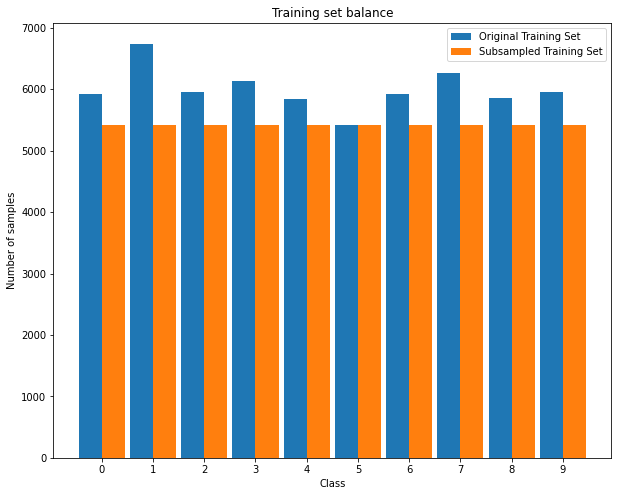
\includegraphics[width=\linewidth]{figures/mnist/training_freq.png}
    \caption{Ιστόγραμμα κλάσεων πριν και μετά την υποδειγματοληψία για τη βάση
    MNIST}
    \label{fig:hist1}
    \end{subfigure}
    \begin{subfigure}[t]{0.48\linewidth}
    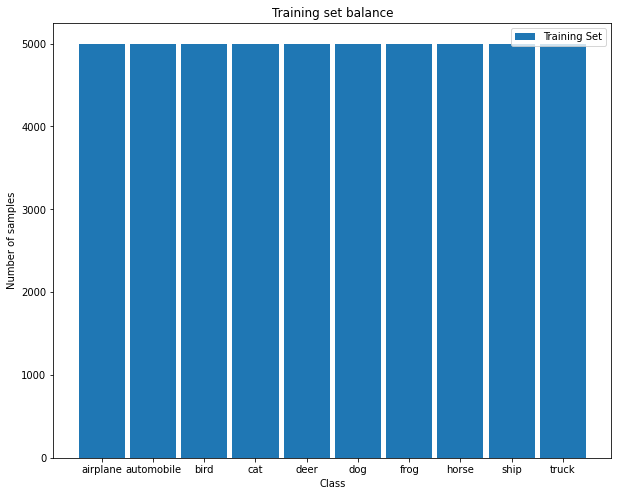
\includegraphics[width=\linewidth]{figures/cifar/training_freq.png}
    \caption{Ιστόγραμμα κλάσεων για τη βάση Cifar-10}
    \end{subfigure}

    \caption{Ιστογράμματα κλάσεων για τις βάσεις δεδομένων}
    \label{fig:hist}
\end{figure}

\end{frame}

\begin{frame}
\frametitle{Προεπεξεργασία δεδομένων}

\begin{block}{Προεπεξεργασία δεδομένων και για τις δύο βάσεις}
\begin{enumerate}
    \item Μετασχηματισμός των δεδομένων στο διάστημα $[0,1]$ για κάθε
        χαρακτηριστικό των δεδομένων.
    \item Εφαρμογή της μεθόδου PCA, κρατώντας τουλάχιστον 90\% της πληροφορίας.
    \item Μετασχηματισμός των δεδομένων στο διάστημα $[0,1]$ για κάθε
        χαρακτηριστικό των δεδομένων ξανά.
\end{enumerate}
\end{block}

\end{frame}

\begin{frame}
\frametitle{Επιλογή παραμέτρων}

\begin{block}{Πυρήνες SVM}
\begin{enumerate}
    \item Γραμμικό SVM
    \item SVM με πολυωνυμικό πυρήνα
    \item SVM με RBF πυρήνα
    \item SVM με σιγμοειδή πυρήνα
\end{enumerate}
\end{block} \pause

Επειδή τα δεδομένα έχουν περισσότερες από δύο κλάσεις (έχουν δέκα),
χρησιμοποιήθηκε η μέθοδος 1vs1 όπου εκπαιδεύονται $\frac{n (n-1)}{2}$ δυαδικοί
ταξινομητές, όπου $n$ ο αριθμός των κλάσεων (δηλαδή 45 δυαδικοί ταξινομητές για
κάθε μοντέλο). Με αυτό τον τρόπο δημιουργούνται όλοι οι δυνατοί συνδυασμοί
δυαδικών ταξινομητών. Οι ταξινομητές αυτοί "ψηφίζουν" ανάμεσα σε δύο κλάσεις
και η τελική κλάση είναι αυτή με τις περισσότερες ψήφους.

\end{frame}

\begin{frame}
\frametitle{Επιλογή παραμέτρων}

Επιπλέον, χρησιμοποιήθηκαν οι μέθοδοι \textbf{πλησιέστερων γειτόνων (Nearest
Neighbors)} και \textbf{πλησιέστερου κέντρου κλάσης (Nearest Class Centroid)},
ώστε να συγκριθούν με τα μοντέλα SVM.


Για κάθε μοντέλο υλοποιήθηκε η μέθοδος \textbf{αναζήτησης πλέγματος (grid
search)} για την εύρεση των καλύτερων παραμέτρων εκτός του μοντέλου πλησιέστερου
κέντρου κλάσης, επειδή ο αλγόριθμος δεν έχει κάποια παράμετρο για επιλογή (εκτός
από την μερική της απόστασης όπου χρησιμοποιήθηκε η ευκλείδεια απόσταση).

\end{frame}

\begin{frame}
\frametitle{Επιλογή παραμέτρων SVM για την MNIST}

Για τη βάση MNIST χρησιμοποιήθηκε 3-fold cross validation για τις παραμέτρους:

\begin{enumerate}
    \item Γραμμικό SVM: $C: (0.1, 1, 10)$
    \item SVM με πολυωνυμικό πυρήνα: $C: (0.1, 1, 10), d: (2, 3, 4), \gamma:
        (0.1, 1, 10)$
    \item SVM με RBF πυρήνα: $C: (1, 10, 50), \gamma: (0.01, 0.1, 1, 10, 100)$
    \item SVM με σιγμοειδή πυρήνα: $C: (10, 100, 1000, 10000), \gamma: (0.0001,
        0.001, 0.01, 0.1)$
\end{enumerate}

\end{frame}

\begin{frame}
\frametitle{Επιλογή παραμέτρων SVM για την Cifar-10}

Για τη βάση Cifar-10 χρησιμοποιήθηκε 2-fold cross validation για τις
παραμέτρους:

\begin{enumerate}
    \item Γραμμικό SVM: $C: (0.1, 1, 10)$
    \item SVM με πολυωνυμικό πυρήνα: $C: (0.1, 1, 10), d: (2, 3), \gamma:
        (0.1, 1)$
    \item SVM με RBF πυρήνα: $C: (1, 10, 50), \gamma: (0.1, 1, 10)$
    \item SVM με σιγμοειδή πυρήνα: $C: (10, 100, 1000), \gamma: (0.0001, 0.001,
        0.01)$
\end{enumerate}

\end{frame}

\begin{frame}
\frametitle{Επεξήγηση παραμέτρων}

Όπου $C$ είναι η παράμετρος του σφάλματος από της εξίσωση:

\begin{equation*}
\begin{split}
\min_{\bm{w},b,\bm{\xi}} & \frac{1}{2} \bm{w}^T\bm{w} + C \sum_{i} \xi_{i} \\
\text{subject to } & y_i (\bm{w^T} \phi (\bm{x}_i) + b) \ge 1 - \xi_i \\
 & \xi_i \ge 0
\end{split}
\end{equation*}

Επίσης οι υπόλοιπες παράμετροι για κάθε πυρήνα είναι:

\begin{enumerate}
    \item SVM με πολυωνυμικό πυρήνα: $K(\bm{x}_i,\bm{x}_j) = (\gamma \bm{x}_i^T
        \bm{x}_j)^d$
    \item SVM με RBF πυρήνα: $K(\bm{x}_i,\bm{x}_j) = exp(-\gamma
        \norm{\bm{x}_i - \bm{x}_j}^2)$
    \item SVM με σιγμοειδή πυρήνα: $K(\bm{x}_i,\bm{x}_j) = tanh(\gamma
        \bm{x}_i^T \bm{x}_j)$
\end{enumerate}

\end{frame}

\begin{frame}
\frametitle{Επιλογή παραμέτρων}

Για το μοντέλο \textbf{πλησιέστερων γειτόνων} και για τις δύο βάσεις
χρησιμοποιήθηκε \textbf{3-fold cross validation}.

\begin{block}{Παράμετροι πλησιέστερων γειτόνων}
\begin{itemize}
    \item $n\_neighbors: (1, 3, 5, 10, 30, 100, 200)$
    \item $weights: (uniform, distance)$
\end{itemize}
Όπου $n\_neighbors$ ο αριθμός των γειτόνων και $weights$ η χρήση βαρών
($distance$ υπολογισμός βαρών μέσω της ευκλείδειας απόστασης και $uniform$
ομοιόμορφα βάρη).
\end{block} \pause

Η μετρική για την επιλογή των παραμέτρων είναι το \textbf{macro F1-score} δηλαδή
ο μέσος όρος των F1-scores για κάθε κλάση.

\end{frame}

\begin{frame}
\frametitle{Επεξήγηση επιλογής παραμέτρων}

Ο λόγος που επιλέχτηκαν παραπάνω παράμετροι για τη βάση MNIST αλλά και
περισσότερες τιμές στο cross validation είναι ο χρόνος εκτέλεσης των πειραμάτων.
Με τις παραμέτρους αυτές ο χρόνος εκτέλεσης των πειραμάτων για τις δύο βάσεις
είναι παρόμοιος. Η διαφορά μεταξύ 2-fold και 3-fold είναι πολύ μεγαλύτερη από τα
$2/3$ του χρόνου εκτέλεσης γιατί τα πειράματα που τρέχουν έχουν και λιγότερα
δείγματα και ο αλγόριθμος εκπαίδευσης (QP solver της libsvm) έχει πολυπλοκότητα
μεταξύ $O(n_{features} \times n^2_{samples})$ και $O(n_{features} \times
n^3_{samples})$.

\end{frame}

\subsection{Αποτελέσματα}

\begin{frame}
\frametitle{Αποτελέσματα}

Τα πειράματα εκτελέστηκαν στο περιβάλλον του
\href{https://colab.research.google.com/}{Google Colab}. Επίσης, για τις
μετρικές precision, recall και F1 χρησιμοποιήθηκε η macro εκδοχή τους που είναι
ο μέσος όρος των μετρικών αυτών για κάθε κλάση.

\end{frame}

\begin{frame}
\frametitle{Γραμμικό SVM}

Παρατηρείται ότι για το μοντέλο του γραμμικού SVM η καλύτερη παράμετρος του $C$
για τη βάση MNIST είναι {\bf10} ενώ για την βάση Cifar-10 είναι {\bf1}.

\begin{figure}[H]
    \centering

    \begin{subfigure}[t]{0.45\linewidth}
    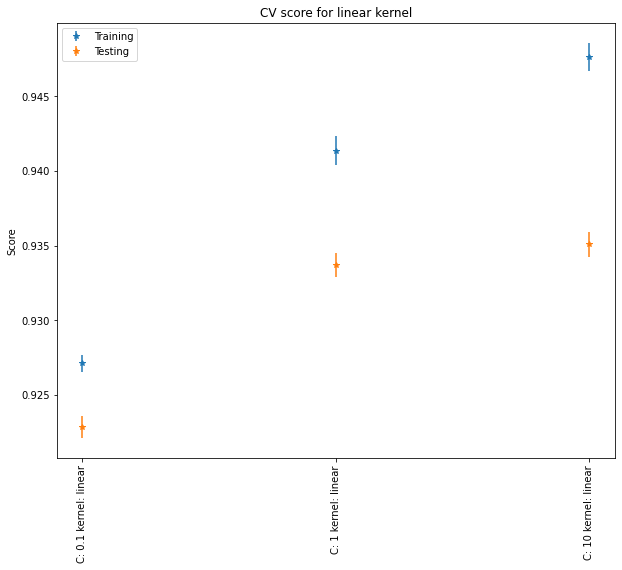
\includegraphics[width=\linewidth]{figures/mnist/cv_results_linear.png}
    \caption{MNIST}
    \end{subfigure}
    \begin{subfigure}[t]{0.45\linewidth}
    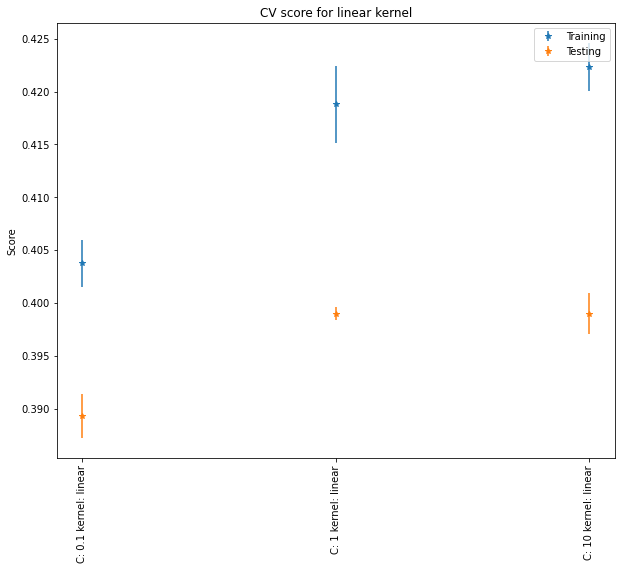
\includegraphics[width=\linewidth]{figures/cifar/cv_results_linear.png}
    \caption{Cifar-10}
    \end{subfigure}

    \caption{Αποτελέσματα αναζήτησης πλέγματος για το γραμμικό SVM}
    \label{fig:cv_linear}
\end{figure}

\end{frame}

\begin{frame}
\frametitle{SVM με πολυωνυμικό πυρήνα}

\begin{figure}[H]
    \centering

    \begin{subfigure}[t]{0.45\linewidth}
    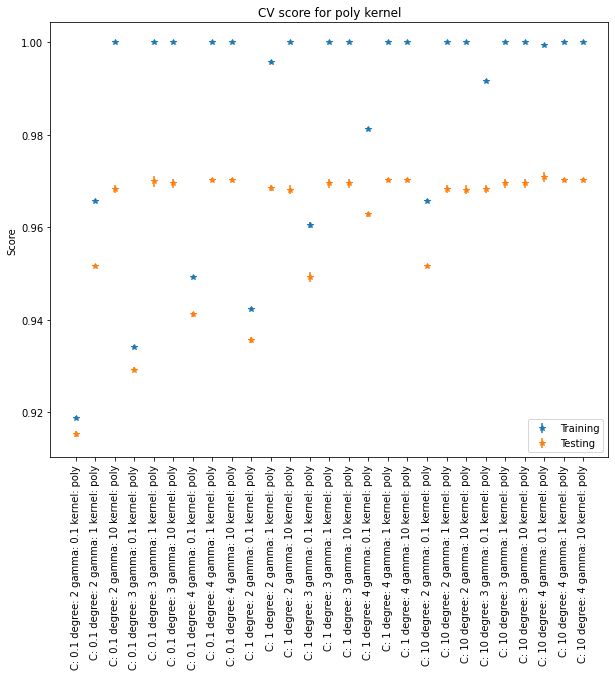
\includegraphics[width=\linewidth]{figures/mnist/cv_results_poly.png}
    \caption{MNIST}
    \end{subfigure}
    \begin{subfigure}[t]{0.45\linewidth}
    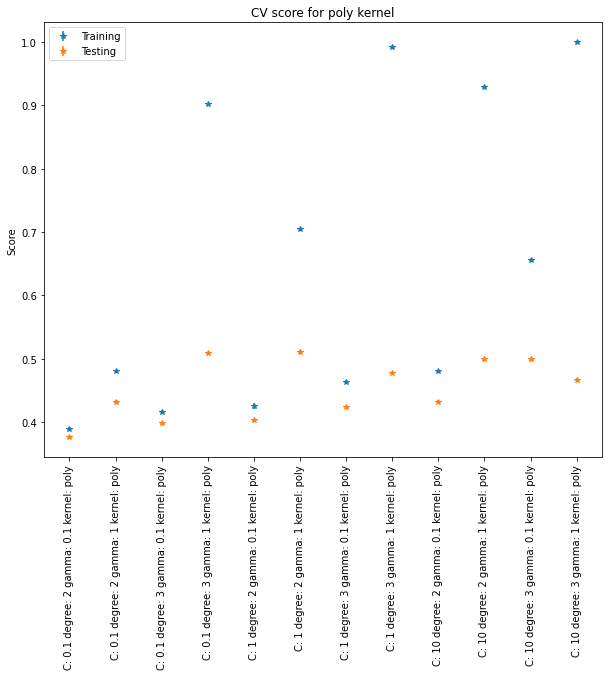
\includegraphics[width=\linewidth]{figures/cifar/cv_results_poly.png}
    \caption{Cifar-10}
    \end{subfigure}

    \caption{Αποτελέσματα αναζήτησης πλέγματος για το SVM με πολυωνυμικό
    πυρήνα}
    \label{fig:cv_poly}
\end{figure}

\end{frame}

\begin{frame}
\frametitle{SVM με πολυωνυμικό πυρήνα}

\begin{table}[h]
\centering
\begin{tabular}{|c|c|c|}
\hline
         & MNIST & Cifar-10 \\ \hline
$C$      & 10    & 1        \\ \hline
$\gamma$ & 0.1   & 1        \\ \hline
$d$      & 4     & 2        \\ \hline
\end{tabular}
\caption{Καλύτεροι παράμετροι SVM με πολυωνυμικό πυρήνα}
\label{tab:best_poly}
\end{table}

\end{frame}

\begin{frame}
\frametitle{SVM με RBF πυρήνα}

\begin{figure}[H]
    \centering

    \begin{subfigure}[t]{0.45\linewidth}
    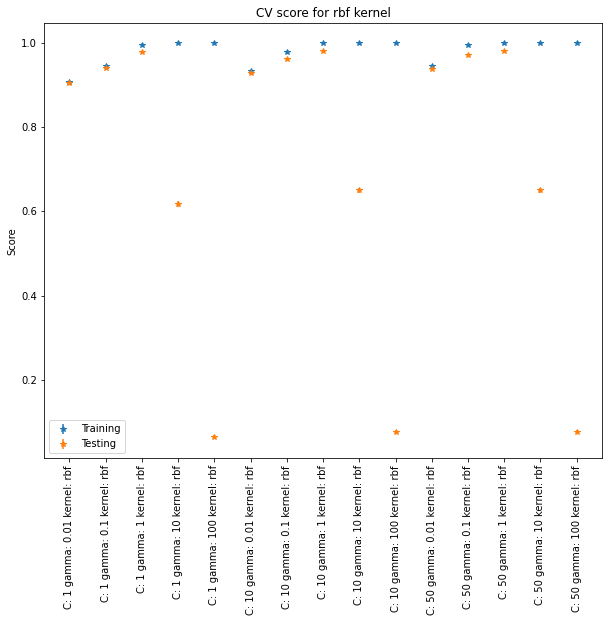
\includegraphics[width=\linewidth]{figures/mnist/cv_results_rbf.png}
    \caption{MNIST}
    \end{subfigure}
    \begin{subfigure}[t]{0.45\linewidth}
    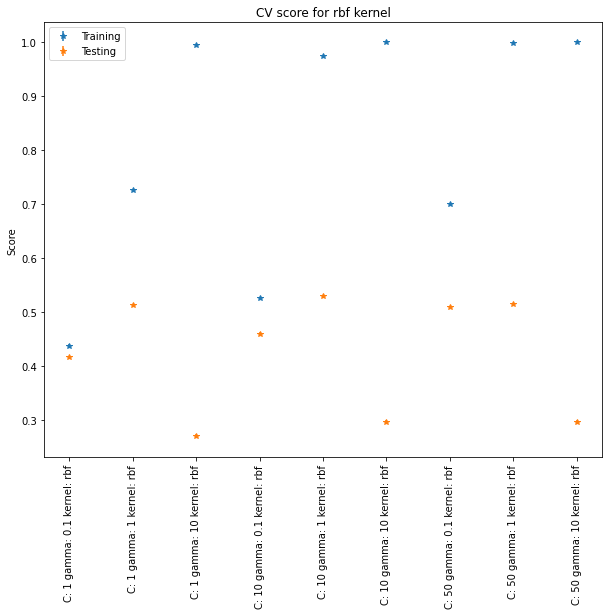
\includegraphics[width=\linewidth]{figures/cifar/cv_results_rbf.png}
    \caption{Cifar-10}
    \end{subfigure}

    \caption{Αποτελέσματα αναζήτησης πλέγματος για το SVM με RBF πυρήνα}
    \label{fig:cv_rbf}
\end{figure}

\end{frame}

\begin{frame}
\frametitle{SVM με RBF πυρήνα}

\begin{table}[h]
\centering
\begin{tabular}{|c|c|c|}
\hline
         & MNIST & Cifar-10 \\ \hline
$C$      & 10    & 10       \\ \hline
$\gamma$ & 1     & 1        \\ \hline
\end{tabular}
\caption{Καλύτεροι παράμετροι SVM με RBF πυρήνα}
\label{tab:best_rbf}
\end{table}

\end{frame}

\begin{frame}
\frametitle{SVM με σιγμοειδή πυρήνα}

\begin{figure}[H]
    \centering

    \begin{subfigure}[t]{0.45\linewidth}
    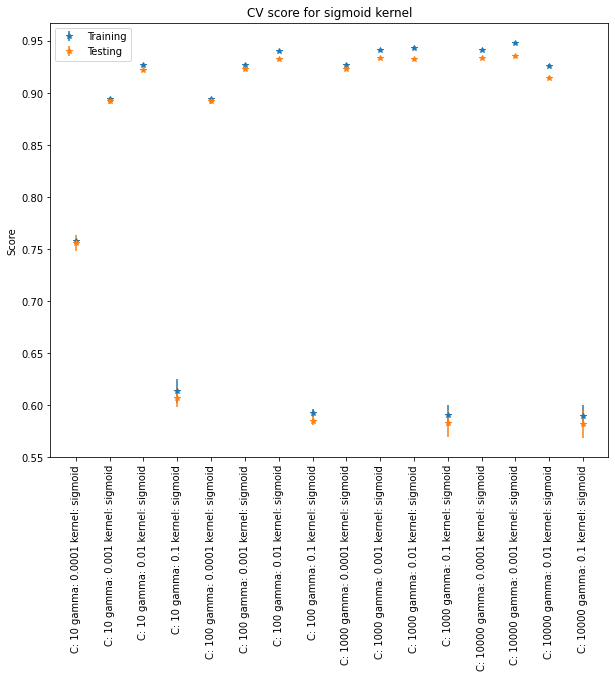
\includegraphics[width=\linewidth]{figures/mnist/cv_results_sigmoid.png}
    \caption{MNIST}
    \end{subfigure}
    \begin{subfigure}[t]{0.45\linewidth}
    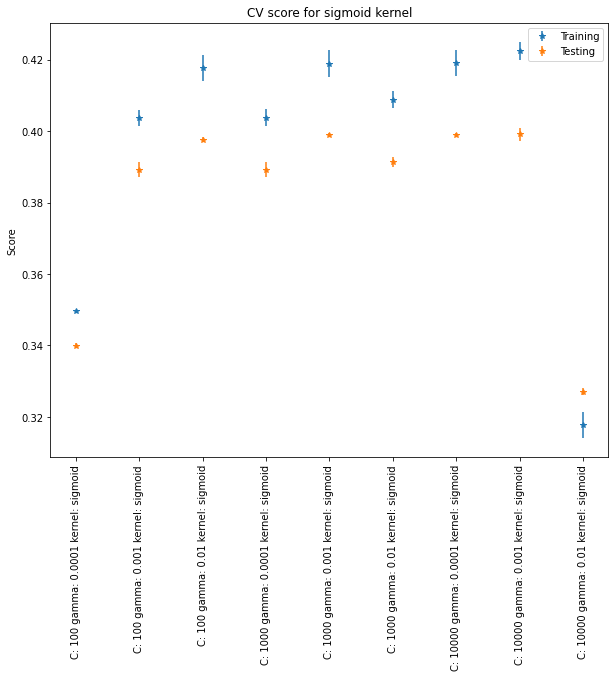
\includegraphics[width=\linewidth]{figures/cifar/cv_results_sigmoid.png}
    \caption{Cifar-10}
    \end{subfigure}

    \caption{Αποτελέσματα αναζήτησης πλέγματος για το SVM με σιγμοειδή πυρήνα}
    \label{fig:cv_sigmoid}
\end{figure}

\end{frame}

\begin{frame}
\frametitle{SVM με σιγμοειδή πυρήνα}

\begin{table}[h]
\centering
\begin{tabular}{|c|c|c|}
\hline
         & MNIST & Cifar-10 \\ \hline
$C$      & 10000 & 10000    \\ \hline
$\gamma$ & 0.001 & 0.001    \\ \hline
\end{tabular}
\caption{Καλύτεροι παράμετροι SVM με σιγμοειδή πυρήνα}
\label{tab:best_sigmoid}
\end{table}

\end{frame}

\begin{frame}
\frametitle{Πλησιέστερων γειτόνων}

\begin{figure}[H]
    \centering

    \begin{subfigure}[t]{0.45\linewidth}
    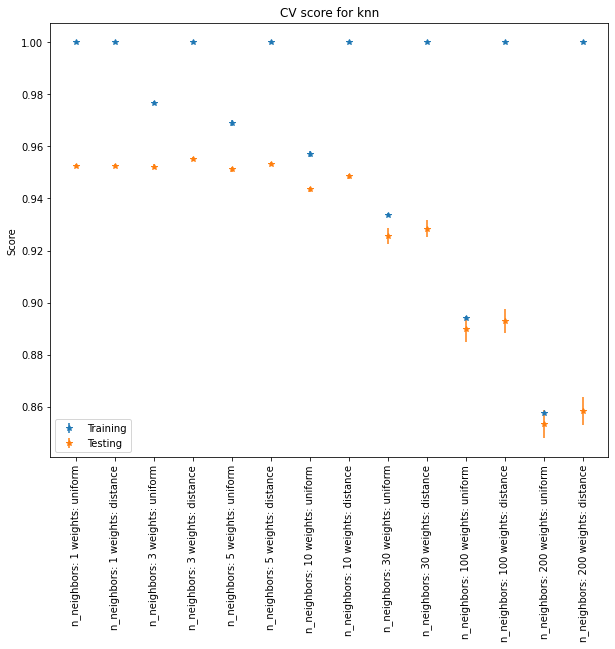
\includegraphics[width=\linewidth]{figures/mnist/cv_results_knn.png}
    \caption{MNIST}
    \end{subfigure}
    \begin{subfigure}[t]{0.45\linewidth}
    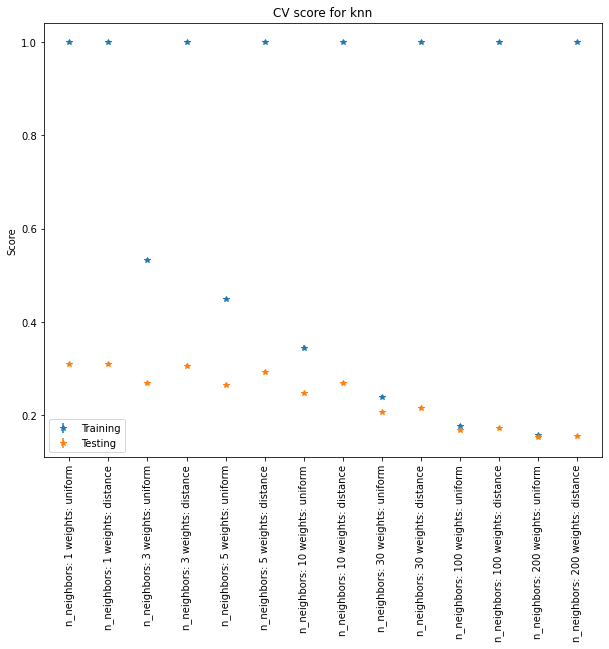
\includegraphics[width=\linewidth]{figures/cifar/cv_results_knn.png}
    \caption{Cifar-10}
    \end{subfigure}

    \caption{Αποτελέσματα αναζήτησης πλέγματος για το μοντέλο πλησιέστερων
    γειτόνων}
    \label{fig:cv_knn}
\end{figure}

\end{frame}

\begin{frame}
\frametitle{Πλησιέστερων γειτόνων}

\begin{table}[h]
\centering
\begin{tabular}{|c|c|c|}
\hline
               & MNIST    & Cifar-10 \\ \hline
$n\_neighbors$ & 3        & 1        \\ \hline
$weights$      & distance & uniform  \\ \hline
\end{tabular}
\caption{Καλύτεροι παράμετροι πλησιέστερων γειτόνων}
\label{tab:best_knn}
\end{table}

\end{frame}

\begin{frame}
\frametitle{Απόδοση μοντέλων στην MNIST}

\tiny
\begin{table}[h]
\begin{tabular}{|l|c|c|c|c|c|}
\hline
\textbf{Model}                                                                        & \textbf{Accuracy} & \textbf{Precision} & \textbf{Recall} & \textbf{F1} & \textbf{Training Time (seconds)} \\ \hline
\begin{tabular}[c]{@{}l@{}}C: 10\\ kernel: linear\end{tabular}                        & 0,9461            & 0,946              & 0,9461          & 0,946       & 57,5676                          \\ \hline
\begin{tabular}[c]{@{}l@{}}C: 10\\ degree: 4\\ gamma: 0.1\\ kernel: poly\end{tabular} & 0,9993            & 0,9993             & 0,9993          & 0,9993      & 54,2103                          \\ \hline
\begin{tabular}[c]{@{}l@{}}C: 10\\ gamma: 1\\ kernel: rbf\end{tabular}                & 1                 & 1                  & 1               & 1           & 125,2382                         \\ \hline
\begin{tabular}[c]{@{}l@{}}C: 10000\\ gamma: 0.001\\ kernel: sigmoid\end{tabular}     & 0,946             & 0,9459             & 0,946           & 0,9459      & 63,1962                          \\ \hline
\begin{tabular}[c]{@{}l@{}}n\_neighbors: 3\\ weights: distance\end{tabular}           & 1                 & 1                  & 1               & 1           & 0,0161                           \\ \hline
Nearest Centroid                                                                      & 0,8495            & 0,852              & 0,8495          & 0,8496      & 0,0508                           \\ \hline
\end{tabular}
\centering
\caption{Μετρικές αποτελεσμάτων στο σύνολο εκπαίδευσης και χρόνος εκπαίδευσης
    για τη βάση MNIST}
\label{tab:mnist_train}
\end{table}

\end{frame}

\begin{frame}
\frametitle{Απόδοση μοντέλων στην MNIST}

\tiny
\begin{table}[h]
\begin{tabular}{|l|c|c|c|c|c|}
\hline
\textbf{Model}                                                                        & \textbf{Accuracy} & \textbf{Precision} & \textbf{Recall} & \textbf{F1} \\ \hline
\begin{tabular}[c]{@{}l@{}}C: 10\\ kernel: linear\end{tabular}                        & 0,9436            & 0,9429             & 0,9428          & 0,9427      \\ \hline
\begin{tabular}[c]{@{}l@{}}C: 10\\ degree: 4\\ gamma: 0.1\\ kernel: poly\end{tabular} & 0,9777            & 0,9776             & 0,9775          & 0,9776      \\ \hline
\begin{tabular}[c]{@{}l@{}}C: 10\\ gamma: 1\\ kernel: rbf\end{tabular}                & 0,9841            & 0,984              & 0,9841          & 0,984       \\ \hline
\begin{tabular}[c]{@{}l@{}}C: 10000\\ gamma: 0.001\\ kernel: sigmoid\end{tabular}     & 0,9437            & 0,943              & 0,9429          & 0,9428      \\ \hline
\begin{tabular}[c]{@{}l@{}}n\_neighbors: 3\\ weights: distance\end{tabular}           & 0,9579            & 0,9584             & 0,9575          & 0,9576      \\ \hline
Nearest Centroid                                                                      & 0,8606            & 0,8614             & 0,859           & 0,8594      \\ \hline
\end{tabular}
\centering
\caption{Μετρικές αποτελεσμάτων στο σύνολο ελέγχο για τη βάση MNIST}
\label{tab:mnist_test}
\end{table}

\end{frame}

\begin{frame}
\frametitle{Απόδοση μοντέλων στην MNIST}

\begin{figure}[H]
    \centering
    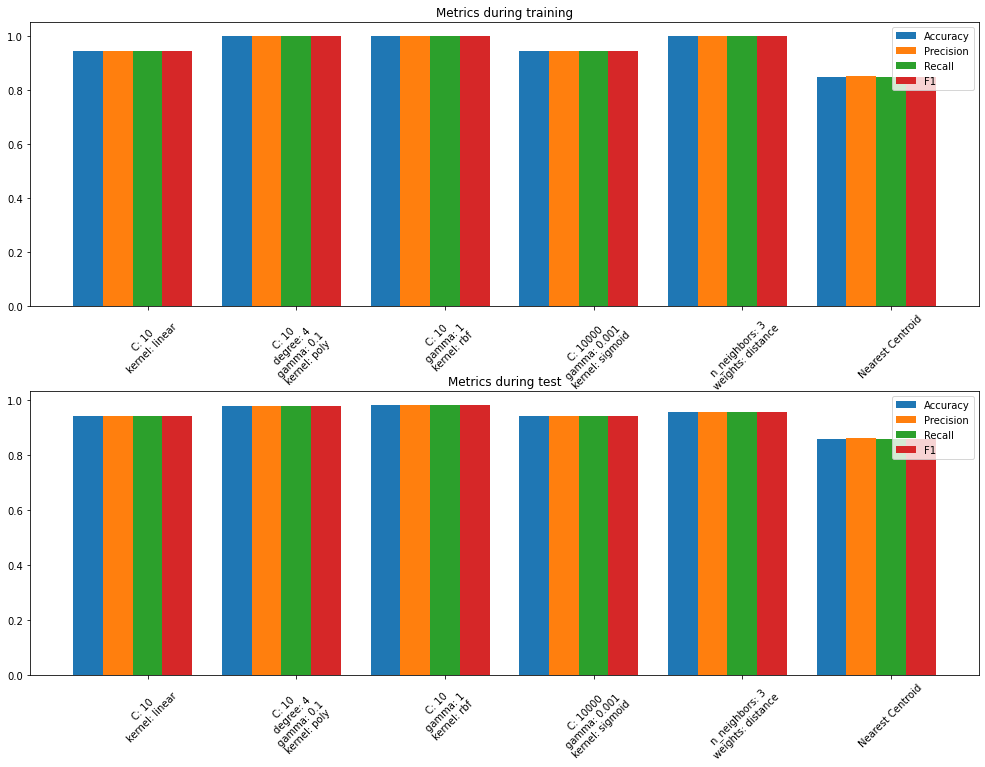
\includegraphics[width=0.8\linewidth]{figures/mnist/all_metrics.png}
    \caption{Μετρικές για τη βάση MNIST}
    \label{fig:mnist_metrics}
\end{figure}

\end{frame}

\begin{frame}
\frametitle{Απόδοση μοντέλων στην MNIST}

\begin{figure}[H]
    \centering
    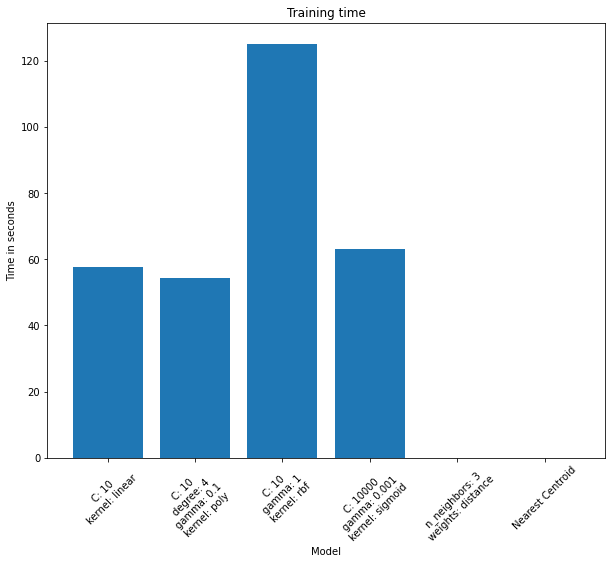
\includegraphics[width=0.6\linewidth]{figures/mnist/training_time.png}
    \caption{Χρόνος εκπαίδευσης για τη βάση MNIST}
    \label{fig:mnist_training_times}
\end{figure}

\end{frame}

\begin{frame}
\frametitle{Απόδοση μοντέλων στην Cifar-10}

\tiny
\begin{table}[h]
\begin{tabular}{|l|c|c|c|c|c|}
\hline
\textbf{Model}                                                                     & \textbf{Accuracy} & \textbf{Precision} & \textbf{Recall} & \textbf{F1} & \textbf{Training Time (seconds)} \\ \hline
\begin{tabular}[c]{@{}l@{}}C: 1\\ kernel: linear\end{tabular}                      & 0,4189            & 0,416              & 0,4189          & 0,416       & 410,7339                         \\ \hline
\begin{tabular}[c]{@{}l@{}}C: 1\\ degree: 2\\ gamma: 1\\ kernel: poly\end{tabular} & 0,6943            & 0,6989             & 0,6943          & 0,695       & 823,6295                         \\ \hline
\begin{tabular}[c]{@{}l@{}}C: 10\\ gamma: 1\\ kernel: rbf\end{tabular}             & 0,9631            & 0,964              & 0,9631          & 0,9634      & 569,9598                         \\ \hline
\begin{tabular}[c]{@{}l@{}}C: 10000\\ gamma: 0.001\\ kernel: sigmoid\end{tabular}  & 0,4204            & 0,4175             & 0,4204          & 0,4175      & 603,1902                         \\ \hline
\begin{tabular}[c]{@{}l@{}}n\_neighbors: 1\\ weights: uniform\end{tabular}         & 1                 & 1                  & 1               & 1           & 0,0092                           \\ \hline
Nearest Centroid                                                                   & 0,3661            & 0,3626             & 0,3661          & 0,3575      & 0,0291                           \\ \hline
\end{tabular}
\centering
\caption{Μετρικές αποτελεσμάτων στο σύνολο εκπαίδευσης και χρόνος εκπαίδευσης
    για τη βάση Cifar-10.}
\label{tab:cifar_train}
\end{table}

\end{frame}

\begin{frame}
\frametitle{Απόδοση μοντέλων στην Cifar-10}

\tiny
\begin{table}[h]
\begin{tabular}{|l|c|c|c|c|c|}
\hline
\textbf{Model}                                                                     & \textbf{Accuracy} & \textbf{Precision} & \textbf{Recall} & \textbf{F1} \\ \hline
\begin{tabular}[c]{@{}l@{}}C: 1\\ kernel: linear\end{tabular}                      & 0,4092            & 0,4067             & 0,4092          & 0,4067      \\ \hline
\begin{tabular}[c]{@{}l@{}}C: 1\\ degree: 2\\ gamma: 1\\ kernel: poly\end{tabular} & 0,5463            & 0,5485             & 0,5463          & 0,5457      \\ \hline
\begin{tabular}[c]{@{}l@{}}C: 10\\ gamma: 1\\ kernel: rbf\end{tabular}             & 0,56              & 0,5626             & 0,56            & 0,5607      \\ \hline
\begin{tabular}[c]{@{}l@{}}C: 10000\\ gamma: 0.001\\ kernel: sigmoid\end{tabular}  & 0,4074            & 0,4046             & 0,4074          & 0,4048      \\ \hline
\begin{tabular}[c]{@{}l@{}}n\_neighbors: 1\\ weights: uniform\end{tabular}         & 0,3394            & 0,4238             & 0,3394          & 0,3307      \\ \hline
Nearest Centroid                                                                   & 0,369             & 0,3647             & 0,369           & 0,3601      \\ \hline
\end{tabular}
\centering
\caption{Μετρικές αποτελεσμάτων στο σύνολο ελέγχο για τη βάση Cifar-10}
\label{tab:cifar_test}
\end{table}

\end{frame}

\begin{frame}
\frametitle{Απόδοση μοντέλων στην Cifar-10}

\begin{figure}[H]
    \centering
    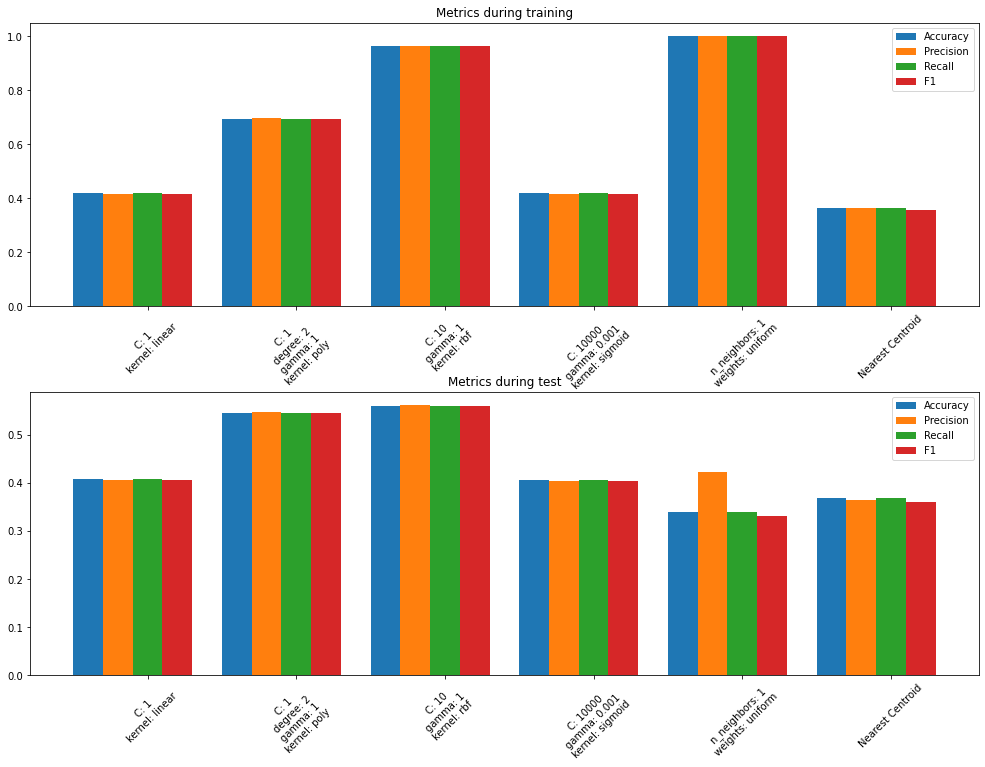
\includegraphics[width=.8\linewidth]{figures/cifar/all_metrics.png}
    \caption{Μετρικές για τη βάση Cifar-10}
    \label{fig:cifar_metrics}
\end{figure}

\end{frame}

\begin{frame}
\frametitle{Απόδοση μοντέλων στην Cifar-10}

\begin{figure}[H]
    \centering
    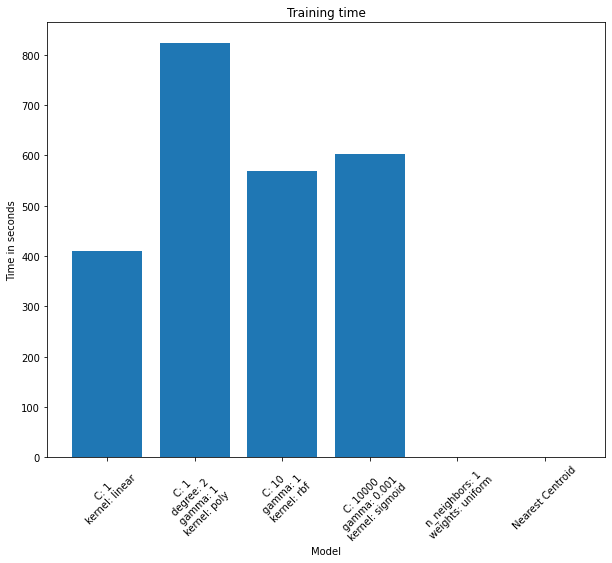
\includegraphics[width=0.6\linewidth]{figures/cifar/training_time.png}
    \caption{Χρόνος εκπαίδευσης για τη βάση Cifar-10}
    \label{fig:cifar_training_times}
\end{figure}

\end{frame}

\begin{frame}
\frametitle{Απόδοση καλύτερου μοντέλου στην MNIST}

\begin{figure}[H]
    \centering
    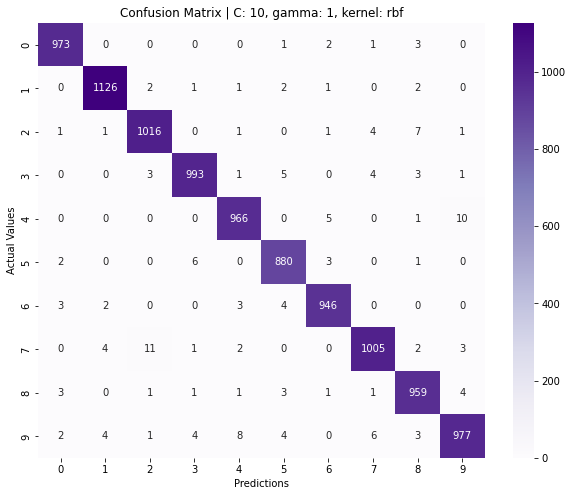
\includegraphics[width=0.6\linewidth]{figures/mnist/confusion_matrix.png}
    \caption{Confusion matrix για τη βάση MNIST}
    \label{fig:mnist_confusion}
\end{figure}

\end{frame}

\begin{frame}
\frametitle{Απόδοση καλύτερου μοντέλου στην MNIST}

\begin{figure}[H]
    \centering

    \begin{subfigure}[t]{0.48\linewidth}
    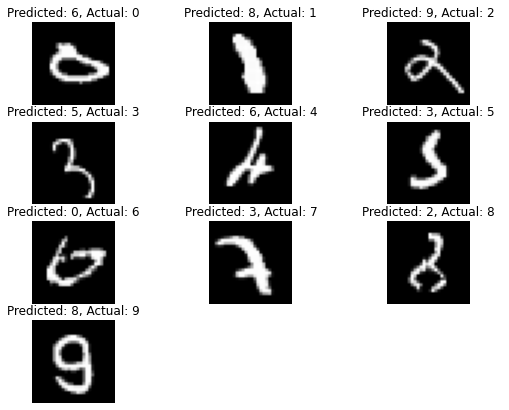
\includegraphics[width=\linewidth]{figures/mnist/wrong_results_1.png}
    \end{subfigure}
    \begin{subfigure}[t]{0.48\linewidth}
    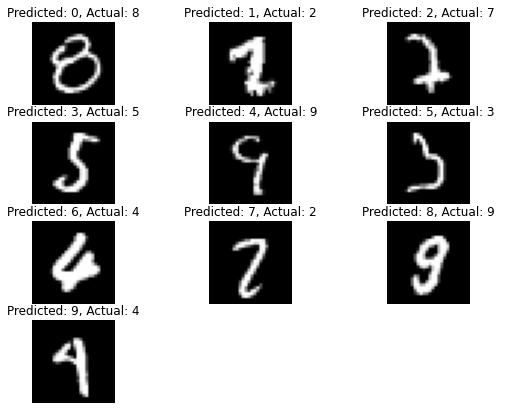
\includegraphics[width=\linewidth]{figures/mnist/wrong_results_2.png}
    \end{subfigure}

    \caption{Λάθος ταξινομήσεις του καλύτερου μοντέλου για τη βάση MNIST}
    \label{fig:mnist_wrong}
\end{figure}

\end{frame}

\begin{frame}
\frametitle{Απόδοση καλύτερου μοντέλου στην Cifar-10}

\begin{figure}[H]
    \centering
    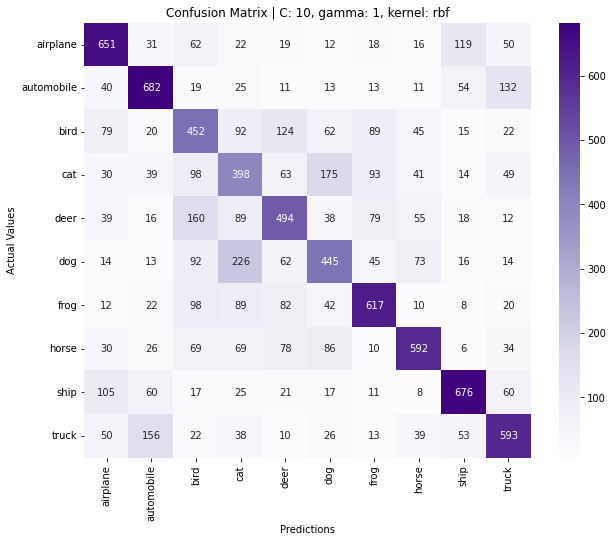
\includegraphics[width=0.6\linewidth]{figures/cifar/confusion_matrix.png}
    \caption{Confusion matrix για τη βάση Cifar-10}
    \label{fig:cifar_confusion}
\end{figure}

\end{frame}

\begin{frame}
\frametitle{Απόδοση καλύτερου μοντέλου στην Cifar-10}

\begin{figure}[H]
    \centering

    \begin{subfigure}[t]{0.48\linewidth}
    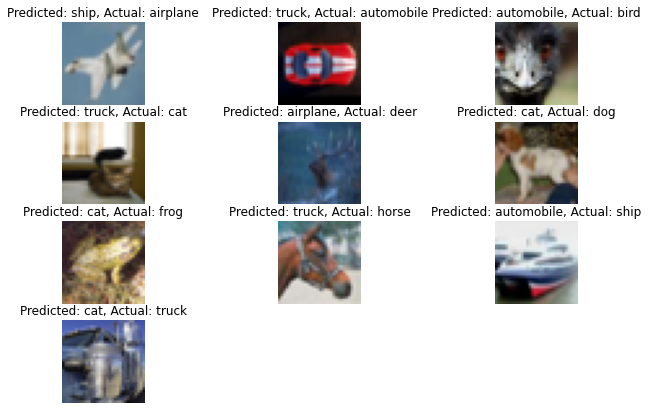
\includegraphics[width=\linewidth]{figures/cifar/wrong_results_1.png}
    \end{subfigure}
    \begin{subfigure}[t]{0.48\linewidth}
    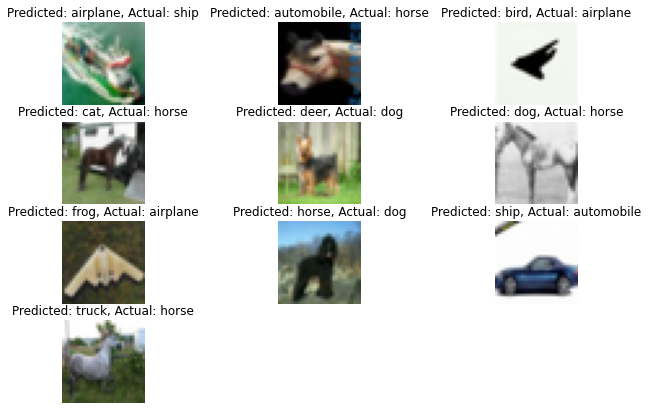
\includegraphics[width=\linewidth]{figures/cifar/wrong_results_2.png}
    \end{subfigure}

    \caption{Λάθος ταξινομήσεις του καλύτερου μοντέλου για τη βάση Cifar-10}
    \label{fig:cifar_wrong}
\end{figure}

\end{frame}


\section{Δεύτερη εργασία}

\subsection{Περιγραφή προβλήματος που επιλέχτηκε}

\begin{frame}
\frametitle{Περιγραφή προβλήματος που επιλέχτηκε}

Οι βάσεις που επιλέχτηκαν, οι οποίες είναι ίδιες με την προηγούμενη εργασία,
είναι:

\begin{enumerate}
\item \href{http://yann.lecun.com/exdb/mnist/}{MNIST}
\item \href{https://www.cs.toronto.edu/~kriz/cifar.html}{Cifar-10}
\end{enumerate}

\end{frame}

\subsection{Υλοποίηση}

\begin{frame}
\frametitle{Επιλογή δειγμάτων}

\begin{figure}[H]
    \centering

    \begin{subfigure}[t]{0.48\linewidth}
    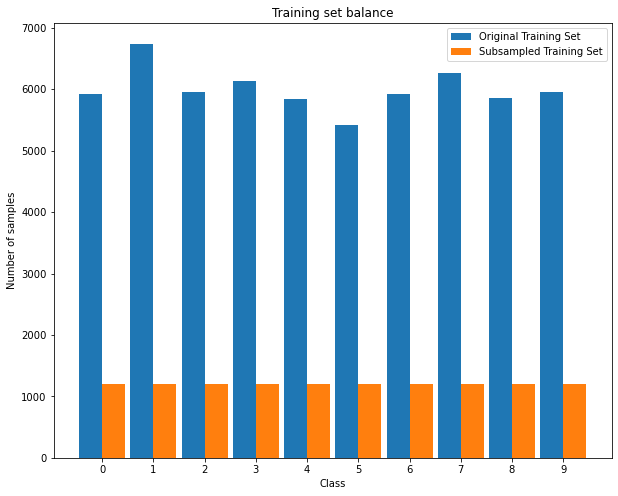
\includegraphics[width=\linewidth]{mnist/training_freq.png}
    \caption{Ιστόγραμμα κλάσεων πριν και μετά την υποδειγματοληψία για τη βάση
    MNIST}
    \label{fig:hist1}
    \end{subfigure}
    \begin{subfigure}[t]{0.48\linewidth}
    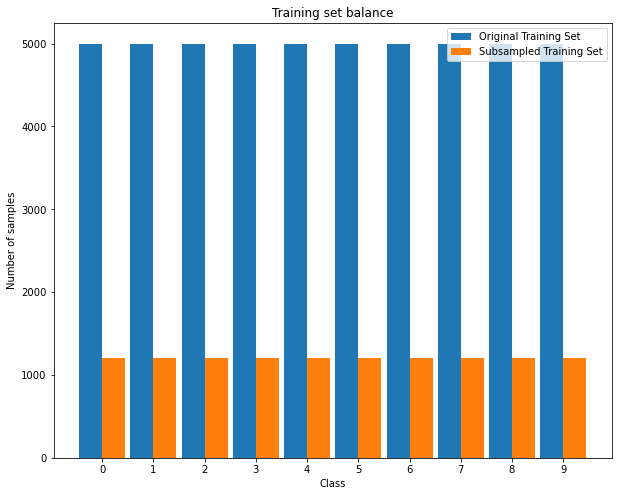
\includegraphics[width=\linewidth]{cifar/training_freq.png}
    \caption{Ιστόγραμμα κλάσεων πριν και μετά την υποδειγματοληψία για τη βάση
        Cifar-10}
    \end{subfigure}

    \caption{Ιστογράμματα κλάσεων για τις βάσεις δεδομένων}
    \label{fig:hist}
\end{figure}

\end{frame}

\begin{frame}
\frametitle{Προεπεξεργασία δεδομένων}

Η μόνη προεπεξεργασία που έγινε στα δεδομένα πριν την χρήση τους στον αλγόριθμο
KPCA plus LDA είναι ο μετασχηματισμός των δεδομένων στο διάστημα $[0,1]$ για
κάθε χαρακτηριστικό των δεδομένων.

\end{frame}

\begin{frame}
\frametitle{Επιλογή παραμέτρων}

Για την εύρεση των καλύτερων παραμέτρων το σύνολο εκπαίδευσης χωρίστηκε σε
σύνολο εκπαίδευσης και επικύρωσης, όπου το σύνολο εκπαίδευσης αποτελείται από
7.000 δείγματα και το σύνολο επικύρωσης από 5.000 δείγματα και για τις δύο
βάσεις.

\end{frame}

\begin{frame}
\frametitle{Επιλογή παραμέτρων}

Για τη βάση MNIST οι παράμετροι είναι:

\begin{enumerate}
    \item Γραμμικός πυρήνας.
    \item Πολυωνυμικός πυρήνας: $d: 2, \gamma: (0.1, 1, 10)$.
    \item RBF πυρήνας: $\gamma: (0.05, 0.1, 0.5)$.
    \item Σιγμοειδής πυρήνας: $\gamma: (0.00001, 0.0001, 0.001$).
\end{enumerate} \pause

Και για τη βάση Cifar-10:

\begin{enumerate}
    \item Γραμμικός πυρήνας.
    \item Πολυωνυμικός πυρήνας: $d: 2, \gamma: (0.01, 0.1, 1)$.
    \item RBF πυρήνας: $\gamma: (0.001, 0.01, 0.1)$.
    \item Σιγμοειδής πυρήνας: $\gamma: (0.00001, 0.0001, 0.001$).
\end{enumerate} \pause

Οι παράμετροι για κάθε πυρήνα είναι:

\begin{enumerate}
    \item Πολυωνυμικός πυρήνας: $K(\bm{x}_i,\bm{x}_j) = (\gamma \bm{x}_i^T
        \bm{x}_j)^d$.
    \item RBF πυρήνας: $K(\bm{x}_i,\bm{x}_j) = exp(-\gamma \norm{\bm{x}_i -
        \bm{x}_j}^2)$.
    \item Σιγμοειδή πυρήνας: $K(\bm{x}_i,\bm{x}_j) = tanh(\gamma \bm{x}_i^T
        \bm{x}_j)$.
\end{enumerate}

\end{frame}

\begin{frame}
\frametitle{Επιλογή παραμέτρων}

Για την ταξινόμηση χρησιμοποιήθηκαν οι μέθοδοι \textbf{πλησιέστερων γειτόνων
(Nearest Neighbors)} και \textbf{πλησιέστερου κέντρου κλάσης (Nearest Class
Centroid)}. Για το μοντέλο πλησιέστερων γειτόνων και για τις δύο βάσεις
χρησιμοποιήθηκε $n\_neighbors: (1, 3, 5, 10, 15)$ όπου $n\_neighbors$ ο αριθμός
των γειτόνων. \pause

Για το μοντέλο \textbf{πλησιέστερων γειτόνων}, για την απόσταση των γειτόνων
χρησιμοποιήθηκε η \textbf{fused απόσταση} που δίνεται στο \cite{kpca_lda} με
$\theta =1$.  Για το μοντέλο του \textbf{πλησιέστερου κέντρου κλάσης}
χρησιμοποιήθηκαν τα \textbf{regular και irregular discriminant features} που
παρουσιάζονται στο \cite{kpca_lda}. Το μέγεθος του διανύσματος των
χαρακτηριστικών είναι 18 από τα οποία 9 αφορούν τα regular και 9 irregular
discriminant features και για τις δύο βάσης.

\end{frame}

\subsection{Αποτελέσματα}

\begin{frame}
\frametitle{Αποτελέσματα}

Τα πειράματα εκτελέστηκαν σε επεξεργαστή Intel i7-4510U και 8GB μνήμη. Επίσης,
για τις μετρικές precision, recall και F1 χρησιμοποιήθηκε η macro εκδοχή τους
που είναι ο μέσος όρος των μετρικών αυτών για κάθε κλάση.

\end{frame}

\begin{frame}
\frametitle{Επιλογή παραμέτρων πλησιέστερων γειτόνων\\ στην MNIST}

\tiny
\begin{table}[H]
\centering
\begin{tabular}{|l|c|c|c|c|c|}
\hline
\textbf{Model}                                                                & \textbf{Best n} & \textbf{Accuracy} & \textbf{Precision} & \textbf{Recall} & \textbf{F1} \\ \hline
kernel: linear                                                                & 1               & 0,1               & 0,01               & 0,1             & 0,0182      \\ \hline
\begin{tabular}[c]{@{}l@{}}kernel: poly\\ degree: 2\\ gamma: 0.1\end{tabular} & 1               & 0,2468            & 0,2038             & 0,2468          & 0,1831      \\ \hline
\begin{tabular}[c]{@{}l@{}}kernel: poly\\ degree: 2\\ gamma: 1\end{tabular}   & 3               & 0,2944            & 0,3749             & 0,2944          & 0,23        \\ \hline
\begin{tabular}[c]{@{}l@{}}kernel: poly\\ degree: 2\\ gamma: 10\end{tabular}  & 1               & 0,1               & 0,01               & 0,1             & 0,0182      \\ \hline
\begin{tabular}[c]{@{}l@{}}kernel: rbf\\ gamma: 0.05\end{tabular}             & 1               & 0,965             & 0,9652             & 0,965           & 0,965       \\ \hline
\begin{tabular}[c]{@{}l@{}}kernel: rbf\\ gamma: 0.1\end{tabular}              & 1               & 0,8762            & 0,9264             & 0,8762          & 0,8892      \\ \hline
\begin{tabular}[c]{@{}l@{}}kernel: rbf\\ gamma: 0.5\end{tabular}              & 10              & 0,2628            & 0,9015             & 0,2628          & 0,2604      \\ \hline
\begin{tabular}[c]{@{}l@{}}kernel: sigmoid\\ gamma: 1e-05\end{tabular}        & 3               & 0,1002            & 0,06               & 0,1002          & 0,0186      \\ \hline
\begin{tabular}[c]{@{}l@{}}kernel: sigmoid\\ gamma: 0.0001\end{tabular}       & 1               & 0,1               & 0,01               & 0,1             & 0,0182      \\ \hline
\begin{tabular}[c]{@{}l@{}}kernel: sigmoid\\ gamma: 0.001\end{tabular}        & 3               & 0,1574            & 0,0812             & 0,1574          & 0,0829      \\ \hline
\end{tabular}
\caption{Αποτελέσματα επιλογής παραμέτρων για την μέθοδο πλησιέστερων γειτόνων
    και τη βάση MNIST}
\label{tab:mnist_knn_val}
\end{table}

\end{frame}

\begin{frame}
\frametitle{Επιλογή παραμέτρων πλησιέστερου κέντρου\\ κλάσης στην MNIST}

\tiny
\begin{table}[H]
\centering
\begin{tabular}{|l|c|c|c|c|}
\hline
\textbf{Model}                                                                & \textbf{Accuracy} & \textbf{Precision} & \textbf{Recall} & \textbf{F1} \\ \hline
kernel: linear                                                                & 0,195             & 0,1683             & 0,195           & 0,098       \\ \hline
\begin{tabular}[c]{@{}l@{}}kernel: poly\\ degree: 2\\ gamma: 0.1\end{tabular} & 0,9156            & 0,9254             & 0,9156          & 0,9161      \\ \hline
\begin{tabular}[c]{@{}l@{}}kernel: poly\\ degree: 2\\ gamma: 1\end{tabular}   & 0,7542            & 0,8715             & 0,7542          & 0,7506      \\ \hline
\begin{tabular}[c]{@{}l@{}}kernel: poly\\ degree: 2\\ gamma: 10\end{tabular}  & 0,1               & 0,01               & 0,1             & 0,0182      \\ \hline
\begin{tabular}[c]{@{}l@{}}kernel: rbf\\ gamma: 0.05\end{tabular}             & 0,9292            & 0,932              & 0,9292          & 0,9299      \\ \hline
\begin{tabular}[c]{@{}l@{}}kernel: rbf\\ gamma: 0.1\end{tabular}              & 0,6912            & 0,8712             & 0,6912          & 0,7356      \\ \hline
\begin{tabular}[c]{@{}l@{}}kernel: rbf\\ gamma: 0.5\end{tabular}              & 0,1526            & 0,1723             & 0,1526          & 0,0916      \\ \hline
\begin{tabular}[c]{@{}l@{}}kernel: sigmoid\\ gamma: 1e-05\end{tabular}        & 0,1152            & 0,206              & 0,1152          & 0,0453      \\ \hline
\begin{tabular}[c]{@{}l@{}}kernel: sigmoid\\ gamma: 0.0001\end{tabular}       & 0,1278            & 0,1024             & 0,1278          & 0,0614      \\ \hline
\begin{tabular}[c]{@{}l@{}}kernel: sigmoid\\ gamma: 0.001\end{tabular}        & 0,133             & 0,2562             & 0,133           & 0,0739      \\ \hline
\end{tabular}
\caption{Αποτελέσματα επιλογής παραμέτρων για την μέθοδο πλησιέστερου κέντρου
    κλάσης και τη βάση MNIST}
\label{tab:mnist_nc_val}
\end{table}

\end{frame}

\begin{frame}
\frametitle{Επιλογή παραμέτρων πλησιέστερων γειτόνων\\ στην Cifar-10}

\tiny
\begin{table}[H]
\centering
\begin{tabular}{|l|c|c|c|c|c|}
\hline
\textbf{Model}                                                                 & \textbf{Best n} & \textbf{Accuracy} & \textbf{Precision} & \textbf{Recall} & \textbf{F1} \\ \hline
kernel: linear                                                                 & 1               & 0,1               & 0,01               & 0,1             & 0,0182      \\ \hline
\begin{tabular}[c]{@{}l@{}}kernel: poly\\ degree: 2\\ gamma: 0.01\end{tabular} & 1               & 0,1               & 0,01               & 0,1             & 0,0182      \\ \hline
\begin{tabular}[c]{@{}l@{}}kernel: poly\\ degree: 2\\ gamma: 0.1\end{tabular}  & 3               & 0,1058            & 0,0278             & 0,1058          & 0,029       \\ \hline
\begin{tabular}[c]{@{}l@{}}kernel: poly\\ degree: 2\\ gamma: 1\end{tabular}    & 1               & 0,1               & 0,01               & 0,1             & 0,0182      \\ \hline
\begin{tabular}[c]{@{}l@{}}kernel: rbf\\ gamma: 0.001\end{tabular}             & 1               & 0,1               & 0,01               & 0,1             & 0,0182      \\ \hline
\begin{tabular}[c]{@{}l@{}}kernel: rbf\\ gamma: 0.01\end{tabular}              & 15              & 0,4198            & 0,5173             & 0,4198          & 0,4233      \\ \hline
\begin{tabular}[c]{@{}l@{}}kernel: rbf\\ gamma: 0.1\end{tabular}               & 10              & 0,1868            & 0,3889             & 0,1868          & 0,1686      \\ \hline
\begin{tabular}[c]{@{}l@{}}kernel: sigmoid\\ gamma: 1e-05\end{tabular}         & 1               & 0,1               & 0,01               & 0,1             & 0,0182      \\ \hline
\begin{tabular}[c]{@{}l@{}}kernel: sigmoid\\ gamma: 0.0001\end{tabular}        & 1               & 0,1               & 0,01               & 0,1             & 0,0182      \\ \hline
\begin{tabular}[c]{@{}l@{}}kernel: sigmoid\\ gamma: 0.001\end{tabular}         & 1               & 0,1               & 0,01               & 0,1             & 0,0182      \\ \hline
\end{tabular}
\caption{Αποτελέσματα επιλογής παραμέτρων για την μέθοδο πλησιέστερων γειτόνων
    και τη βάση Cifar-10}
\label{tab:cifar_knn_val}
\end{table}

\end{frame}

\begin{frame}
\frametitle{Επιλογή παραμέτρων πλησιέστερου κέντρου\\ κλάσης στην Cifar-10}

\tiny
\begin{table}[H]
\centering
\begin{tabular}{|l|c|c|c|c|}
\hline
\textbf{Model}                                                                 & \textbf{Accuracy} & \textbf{Precision} & \textbf{Recall} & \textbf{F1} \\ \hline
kernel: linear                                                                 & 0,1246            & 0,027              & 0,1246          & 0,0419      \\ \hline
\begin{tabular}[c]{@{}l@{}}kernel: poly\\ degree: 2\\ gamma: 0.01\end{tabular} & 0,1002            & 0,11               & 0,1002          & 0,0186      \\ \hline
\begin{tabular}[c]{@{}l@{}}kernel: poly\\ degree: 2\\ gamma: 0.1\end{tabular}  & 0,1               & 0,01               & 0,1             & 0,0182      \\ \hline
\begin{tabular}[c]{@{}l@{}}kernel: poly\\ degree: 2\\ gamma: 1\end{tabular}    & 0,1               & 0,01               & 0,1             & 0,0182      \\ \hline
\begin{tabular}[c]{@{}l@{}}kernel: rbf\\ gamma: 0.001\end{tabular}             & 0,146             & 0,1267             & 0,146           & 0,0686      \\ \hline
\begin{tabular}[c]{@{}l@{}}kernel: rbf\\ gamma: 0.01\end{tabular}              & 0,4512            & 0,4597             & 0,4512          & 0,4461      \\ \hline
\begin{tabular}[c]{@{}l@{}}kernel: rbf\\ gamma: 0.1\end{tabular}               & 0,1696            & 0,3601             & 0,1696          & 0,1273      \\ \hline
\begin{tabular}[c]{@{}l@{}}kernel: sigmoid\\ gamma: 1e-05\end{tabular}         & 0,128             & 0,0258             & 0,128           & 0,0427      \\ \hline
\begin{tabular}[c]{@{}l@{}}kernel: sigmoid\\ gamma: 0.0001\end{tabular}        & 0,1               & 0,01               & 0,1             & 0,0182      \\ \hline
\begin{tabular}[c]{@{}l@{}}kernel: sigmoid\\ gamma: 0.001\end{tabular}         & 0,1               & 0,01               & 0,1             & 0,0182      \\ \hline
\end{tabular}
\caption{Αποτελέσματα επιλογής παραμέτρων για την μέθοδο πλησιέστερου κέντρου
    κλάσης και τη βάση Cifar-10}
\label{tab:cifar_nc_val}
\end{table}

\end{frame}

\begin{frame}
\frametitle{Αποτελέσματα πλησιέστερων γειτόνων στην MNIST}

\tiny
\begin{table}[H]
\centering
\begin{tabular}{|l|c|c|c|c|c|c|c|}
\hline
\textbf{Model}                                                    & \textbf{Best n} & \textbf{Accuracy} & \textbf{Precision} & \textbf{Recall} & \textbf{F1} & \textbf{KPCA+LDA Time (seconds)} & \textbf{kNN Time} \\ \hline
\begin{tabular}[c]{@{}l@{}}kernel: rbf\\ gamma: 0.05\end{tabular} & 1               & 1                 & 1                  & 1               & 1           & 8818,2817                        & 2,8122            \\ \hline
\end{tabular}
\caption{Αποτελέσματα καλύτερου μοντέλου πλησιέστερων γειτόνων στο σύνολο
    εκπαίδευσης για τη βάση MNIST}
\label{tab:mnist_train_final_knn}
\end{table}

\begin{table}[H]
\centering
\begin{tabular}{|l|c|c|c|c|c|c|c|}
\hline
\textbf{Model}                                                    & \textbf{Best n} & \textbf{Accuracy} & \textbf{Precision} & \textbf{Recall} & \textbf{F1} & \textbf{KPCA+LDA Time (seconds)} & \textbf{kNN Time} \\ \hline
\begin{tabular}[c]{@{}l@{}}kernel: rbf\\ gamma: 0.05\end{tabular} & 1               & 0,9726            & 0,9726             & 0,9726          & 0,9725      & 8818,2817                        & 2,8122            \\ \hline
\end{tabular}
\caption{Αποτελέσματα καλύτερου μοντέλου πλησιέστερων γειτόνων στο σύνολο
    ελέγχου για τη βάση MNIST}
\label{tab:mnist_test_final_knn}
\end{table}

\end{frame}


\begin{frame}
\frametitle{Αποτελέσματα πλησιέστερων γειτόνων στην MNIST}

\begin{figure}[H]
    \centering
    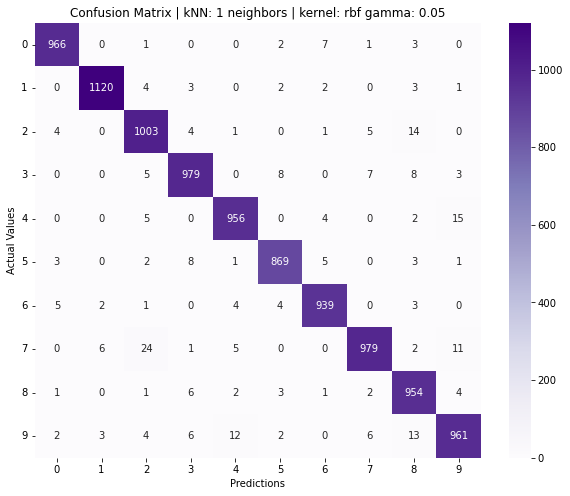
\includegraphics[width=0.6\linewidth]{mnist/confusion_matrix_knn.png}
    \caption{Confusion matrix για τη μέθοδο πλησιέστερων γειτόνων για τη βάση
    MNIST}
    \label{fig:mnist_confusion_knn}
\end{figure}

\end{frame}

\begin{frame}
\frametitle{Αποτελέσματα πλησιέστερων γειτόνων στην MNIST}

\begin{figure}[H]
    \centering

    \begin{subfigure}[t]{0.48\linewidth}
    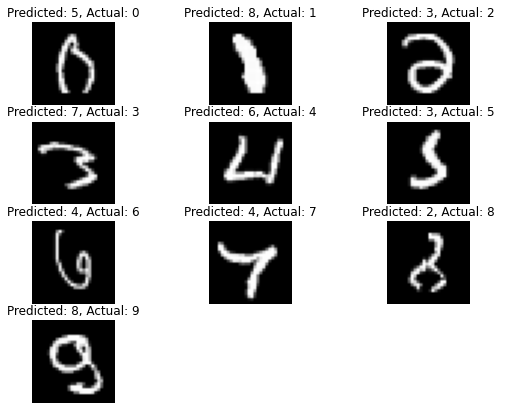
\includegraphics[width=\linewidth]{mnist/wrong_results_knn_1.png}
    \end{subfigure}
    \begin{subfigure}[t]{0.48\linewidth}
    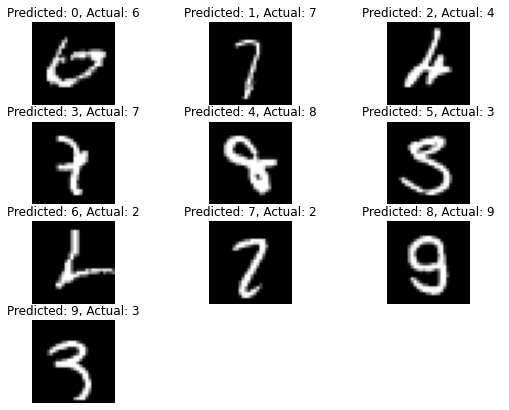
\includegraphics[width=\linewidth]{mnist/wrong_results_knn_2.png}
    \end{subfigure}

    \caption{Λάθος ταξινομήσεις του καλύτερου μοντέλου για τη μέθοδο
    πλησιέστερων γειτόνων και τη βάση MNIST}
    \label{fig:mnist_wrong_knn}
\end{figure}

\end{frame}

\begin{frame}
\frametitle{Αποτελέσματα πλησιέστερου κέντρου κλάσης\\στην MNIST}

\tiny
\begin{table}[H]
\centering
\begin{tabular}{|l|c|c|c|c|c|c|}
\hline
\textbf{Model}                                                    & \textbf{Accuracy} & \textbf{Precision} & \textbf{Recall} & \textbf{F1} & \textbf{KPCA+LDA Time (seconds)} & \textbf{Nearest Centroid Time} \\ \hline
\begin{tabular}[c]{@{}l@{}}kernel: rbf\\ gamma: 0.05\end{tabular} & 0,9145            & 0,9158             & 0,9145          & 0,9149      & 8818,2817                        & 0,0125                         \\ \hline
\end{tabular}
\caption{Αποτελέσματα καλύτερου μοντέλου πλησιέστερου κέντρου κλάσης στο σύνολο
    εκπαίδευσης για τη βάση MNIST}
\label{tab:mnist_train_final_nc}
\end{table}

\begin{table}[H]
\centering
\begin{tabular}{|l|c|c|c|c|c|c|}
\hline
\textbf{Model}                                                    & \textbf{Accuracy} & \textbf{Precision} & \textbf{Recall} & \textbf{F1} & \textbf{KPCA+LDA Time (seconds)} & \textbf{Nearest Centroid Time} \\ \hline
\begin{tabular}[c]{@{}l@{}}kernel: rbf\\ gamma: 0.05\end{tabular} & 0,9484            & 0,9487             & 0,9482          & 0,9482      & 8818,2817                        & 0,0125                         \\ \hline
\end{tabular}
\caption{Αποτελέσματα καλύτερου μοντέλου πλησιέστερου κέντρου κλάσης στο σύνολο
    ελέγχου για τη βάση MNIST}
\label{tab:mnist_test_final_nc}
\end{table}

\end{frame}

\begin{frame}
\frametitle{Αποτελέσματα πλησιέστερου κέντρου κλάσης\\στην MNIST}

\begin{figure}[H]
    \centering
    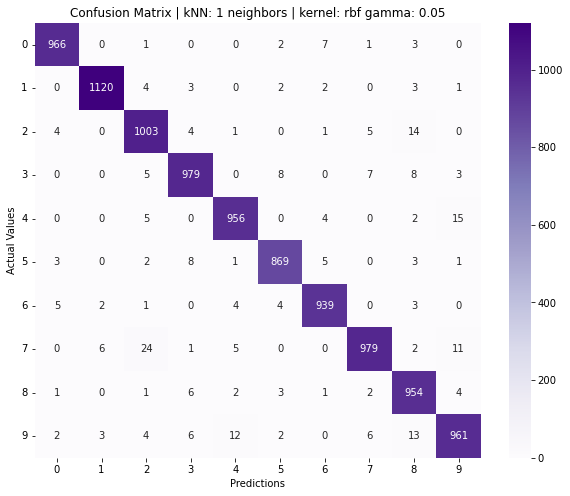
\includegraphics[width=0.6\linewidth]{mnist/confusion_matrix_knn.png}
    \caption{Confusion matrix για τη μέθοδο πλησιέστερου κέντρου κλάσης για τη
    βάση MNIST}
    \label{fig:mnist_confusion_nc}
\end{figure}

\end{frame}

\begin{frame}
\frametitle{Αποτελέσματα πλησιέστερου κέντρου κλάσης\\στην MNIST}

\begin{figure}[H]
    \centering

    \begin{subfigure}[t]{0.48\linewidth}
    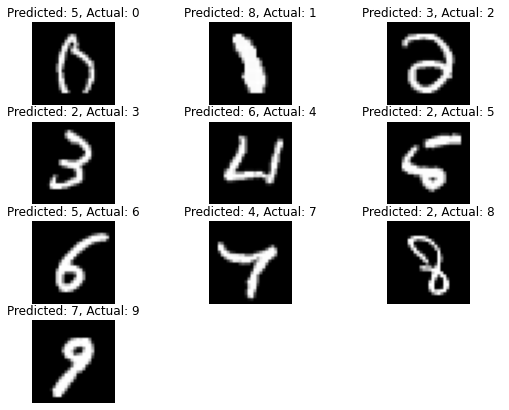
\includegraphics[width=\linewidth]{mnist/wrong_results_nc_1.png}
    \end{subfigure}
    \begin{subfigure}[t]{0.48\linewidth}
    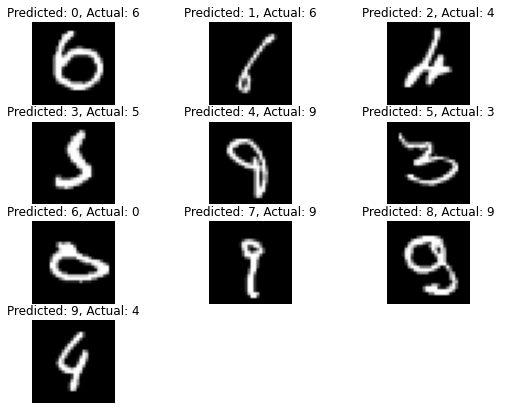
\includegraphics[width=\linewidth]{mnist/wrong_results_nc_2.png}
    \end{subfigure}

    \caption{Λάθος ταξινομήσεις του καλύτερου μοντέλου για τη μέθοδο
    πλησιέστερου κέντρου κλάσης και τη βάση MNIST}
    \label{fig:mnist_wrong_nc}
\end{figure}

\end{frame}

\begin{frame}
\frametitle{Αποτελέσματα πλησιέστερων γειτόνων στην Cifar-10}

\tiny
\begin{table}[H]
\centering
\begin{tabular}{|l|c|c|c|c|c|c|c|}
\hline
\textbf{Model}                                                    & \textbf{Best n} & \textbf{Accuracy} & \textbf{Precision} & \textbf{Recall} & \textbf{F1} & \textbf{KPCA+LDA Time (seconds)} & \textbf{kNN Time} \\ \hline
\begin{tabular}[c]{@{}l@{}}kernel: rbf\\ gamma: 0.01\end{tabular} & 15              & 0,9992            & 0,9992             & 0,9992          & 0,9992      & 13608,5766                       & 5,3204            \\ \hline
\end{tabular}
\caption{Αποτελέσματα καλύτερου μοντέλου πλησιέστερων γειτόνων στο σύνολο
    εκπαίδευσης για τη βάση Cifar-10}
\label{tab:cifar_train_final_knn}
\end{table}

\begin{table}[H]
\centering
\begin{tabular}{|l|c|c|c|c|c|c|c|}
\hline
\textbf{Model}                                                    & \textbf{Best n} & \textbf{Accuracy} & \textbf{Precision} & \textbf{Recall} & \textbf{F1} & \textbf{KPCA+LDA Time (seconds)} & \textbf{kNN Time} \\ \hline
\begin{tabular}[c]{@{}l@{}}kernel: rbf\\ gamma: 0.01\end{tabular} & 15              & 0,449             & 0,5304             & 0,449           & 0,4499      & 13608,5766                       & 5,3204            \\ \hline
\end{tabular}
\caption{Αποτελέσματα καλύτερου μοντέλου πλησιέστερων γειτόνων στο σύνολο
    ελέγχου για τη βάση Cifar-10}
\label{tab:cifar_test_final_knn}
\end{table}

\end{frame}

\begin{frame}
\frametitle{Αποτελέσματα πλησιέστερων γειτόνων στην Cifar-10}

\begin{figure}[H]
    \centering
    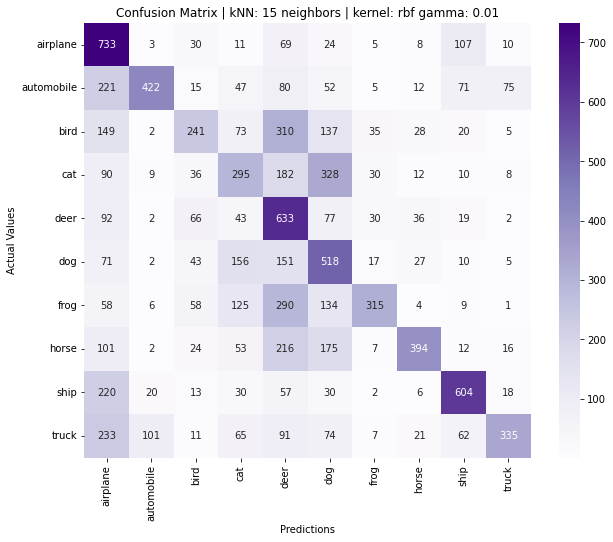
\includegraphics[width=0.6\linewidth]{cifar/confusion_matrix_knn.png}
    \caption{Confusion matrix για τη μέθοδο πλησιέστερων γειτόνων και τη βάση
    Cifar-10}
    \label{fig:cifar_confusion_knn}
\end{figure}

\end{frame}

\begin{frame}
\frametitle{Αποτελέσματα πλησιέστερων γειτόνων στην Cifar-10}

\begin{figure}[H]
    \centering

    \begin{subfigure}[t]{0.48\linewidth}
    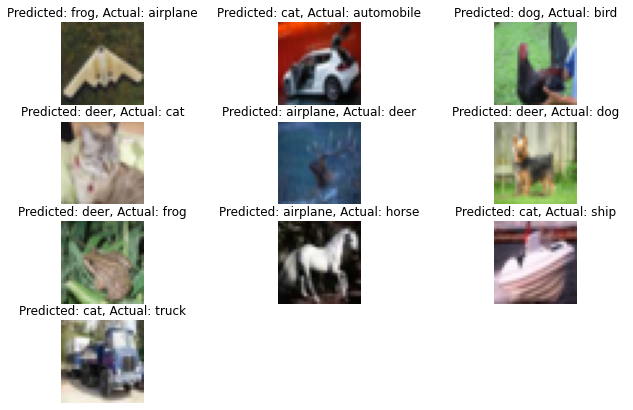
\includegraphics[width=\linewidth]{cifar/wrong_results_knn_1.png}
    \end{subfigure}
    \begin{subfigure}[t]{0.48\linewidth}
    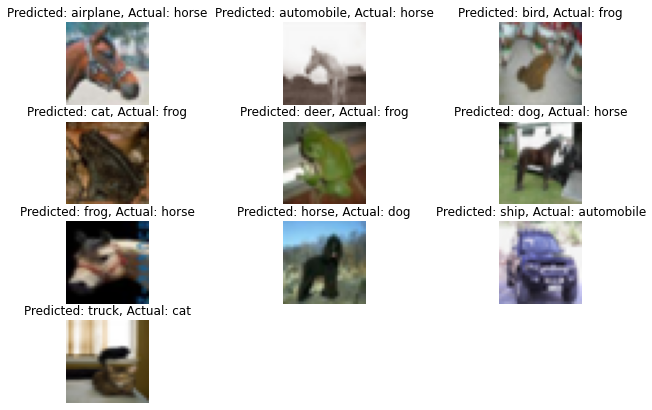
\includegraphics[width=\linewidth]{cifar/wrong_results_knn_2.png}
    \end{subfigure}

    \caption{Λάθος ταξινομήσεις του καλύτερου μοντέλου για τη μέθοδο
    πλησιέστερων γειτόνων και τη βάση Cifar-10}
    \label{fig:cifar_wrong_knn}
\end{figure}

\end{frame}

\begin{frame}
\frametitle{Αποτελέσματα πλησιέστερου κέντρου κλάσης\\στην Cifar-10}

\tiny
\begin{table}[H]
\centering
\begin{tabular}{|l|c|c|c|c|c|c|}
\hline
\textbf{Model}                                                    & \textbf{Accuracy} & \textbf{Precision} & \textbf{Recall} & \textbf{F1} & \textbf{KPCA+LDA Time (seconds)} & \textbf{Nearest Centroid Time} \\ \hline
\begin{tabular}[c]{@{}l@{}}kernel: rbf\\ gamma: 0.01\end{tabular} & 0,7629            & 0,7637             & 0,7629          & 0,7631      & 13608,5766                       & 0,0118                         \\ \hline
\end{tabular}
\caption{Αποτελέσματα καλύτερου μοντέλου πλησιέστερου κέντρου κλάσης στο σύνολο
    εκπαίδευσης για τη βάση Cifar-10}
\label{tab:cifar_train_final_nc}
\end{table}

\begin{table}[H]
\centering
\begin{tabular}{|l|c|c|c|c|c|c|}
\hline
\textbf{Model}                                                    & \textbf{Accuracy} & \textbf{Precision} & \textbf{Recall} & \textbf{F1} & \textbf{KPCA+LDA Time (seconds)} & \textbf{Nearest Centroid Time} \\ \hline
\begin{tabular}[c]{@{}l@{}}kernel: rbf\\ gamma: 0.01\end{tabular} & 0,4866            & 0,4899             & 0,4866          & 0,4808      & 13608,5766                       & 0,0118                         \\ \hline
\end{tabular}
\caption{Αποτελέσματα καλύτερου μοντέλου πλησιέστερου κέντρου κλάσης στο σύνολο
    ελέγχου για τη βάση Cifar-10}
\label{tab:cifar_test_final_nc}
\end{table}

\end{frame}

\begin{frame}
\frametitle{Αποτελέσματα πλησιέστερου κέντρου κλάσης\\στην Cifar-10}

\begin{figure}[H]
    \centering
    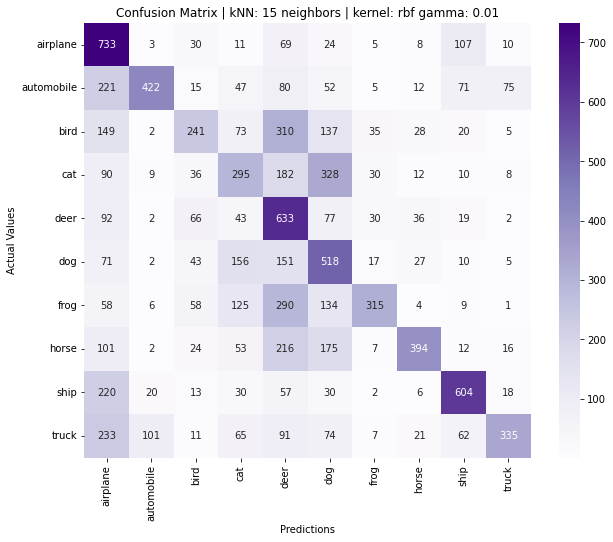
\includegraphics[width=0.6\linewidth]{cifar/confusion_matrix_knn.png}
    \caption{Confusion matrix για τη μέθοδο πλησιέστερου κέντρου κλάσης και τη
    βάση Cifar-10}
    \label{fig:cifar_confusion_nc}
\end{figure}

\end{frame}

\begin{frame}
\frametitle{Αποτελέσματα πλησιέστερου κέντρου κλάσης\\στην Cifar-10}

\begin{figure}[H]
    \centering

    \begin{subfigure}[t]{0.48\linewidth}
    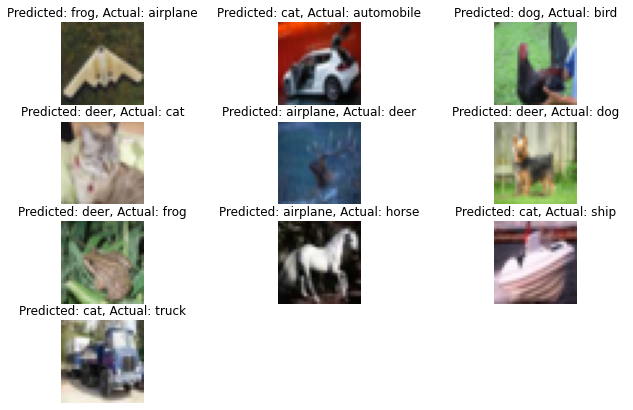
\includegraphics[width=\linewidth]{cifar/wrong_results_knn_1.png}
    \end{subfigure}
    \begin{subfigure}[t]{0.48\linewidth}
    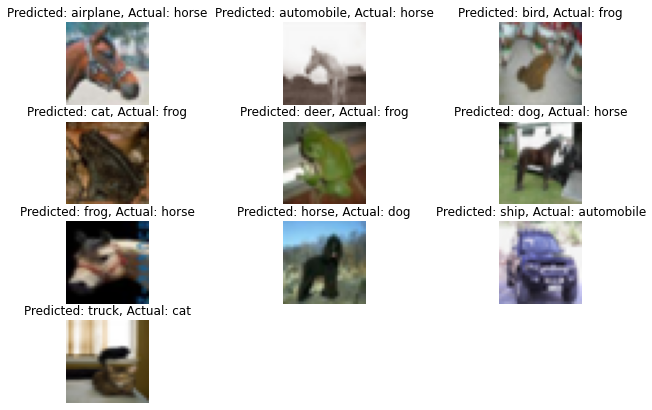
\includegraphics[width=\linewidth]{cifar/wrong_results_knn_2.png}
    \end{subfigure}

    \caption{Λάθος ταξινομήσεις του καλύτερου μοντέλου για τη μέθοδο
    πλησιέστερου κέντρου κλάσης και τη βάση Cifar-10}
    \label{fig:cifar_wrong_nc}
\end{figure}

\end{frame}

\subsection{Σύγκριση με τα αποτελέσματα των SVMs}

\begin{frame}
\frametitle{Σύγκριση με τα αποτελέσματα των SVMs}

\begin{table}[H]
\centering
\begin{tabular}{|l|c|c|c|c|}
\hline
\textbf{Model} & \textbf{Accuracy} & \textbf{Precision} & \textbf{Recall} & \textbf{F1}\\ \hline
SVM & 0,9841 & 0,984 & 0,9841 & 0,984\\ \hline
KPCA+LDA & 0,9726 & 0,9726 & 0,9726 & 0,9725 \\ \hline
\end{tabular}
\caption{Αποτελέσματα για τα καλύτερα μοντέλα για τις αρχιτεκτονικές SVM και
    KPCA plus LDA στο σύνολο ελέγχου για τη βάση MNIST}
\label{tab:mnist_svm_kpca}
\end{table}

\begin{table}[H]
\centering
\begin{tabular}{|l|c|c|c|c|}
\hline
\textbf{Model} & \textbf{Accuracy} & \textbf{Precision} & \textbf{Recall} & \textbf{F1}\\ \hline
SVM & 0,56 & 0,5626 & 0,56 & 0,5607\\ \hline
KPCA+LDA & 0,4866 & 0,4899 & 0,4866 & 0,4808\\ \hline
\end{tabular}
\caption{Αποτελέσματα για τα καλύτερα μοντέλα για τις αρχιτεκτονικές SVM και
    KPCA plus LDA στο σύνολο ελέγχου για τη βάση Cifar-10}
\label{tab:cifar_svm_kpca}
\end{table}

\end{frame}

\section{Τρίτη εργασία}

\subsection{Περιγραφή προβλήματος που επιλέχτηκε}

\begin{frame}
\frametitle{Περιγραφή προβλήματος που επιλέχτηκε}

Οι βάσεις που επιλέχτηκαν, οι οποίες είναι ίδιες με την προηγούμενη εργασία,
είναι:

\begin{enumerate}
\item \href{http://yann.lecun.com/exdb/mnist/}{MNIST}
\item \href{https://www.cs.toronto.edu/~kriz/cifar.html}{Cifar-10}
\end{enumerate}

\end{frame}

\subsection{Υλοποίηση}

\begin{frame}
\frametitle{Προεπεξεργασία δεδομένων}

Η μόνη προεπεξεργασία που έγινε στα δεδομένα πριν την χρήση τους είναι ο
μετασχηματισμός των δεδομένων στο διάστημα $[0,1]$ για κάθε χαρακτηριστικό των
δεδομένων.

\end{frame}

\begin{frame}
\frametitle{Επιλογή παραμέτρων t-SNE}

Και για τις δύο βάσεις ελέγχθηκαν οι τιμές του perplexity $[10, 20, 30, 40, 50,
60]$.

\end{frame}

\begin{frame}
\frametitle{Επιλογή παραμέτρων spectral clustering}

Για τον αλγόριθμο του \textbf{spectral clustering} για τη δημιουργία του
similarity matrix χρησιμοποιήθηκε ο αλγόριθμος των \textbf{πλησιέστερων
γειτόνων} επειδή μπορεί να αναπαρασταθεί με αραιό πίνακα σε σχέση με τις
μεθόδους των πυρήνων. Με αυτό τον τρόπο είναι δυνατό να τρέξει ο αλγόριθμος σε
όλα τα δεδομένα, χωρίς να χρειάζεται πάρα πολύ μνήμη. \pause

Επίσης, για τον αλγόριθμο αυτό χρησιμοποιήθηκε η κανονική μορφή του λαπλασιανού
πίνακα και όχι η κανονικοποιημένη. Ακόμα, επειδή το ιδιοδιάνυσμα που αντιστοιχεί
στην ιδιοτιμή 0 έχει όλες τις τιμές του ίδιες, δεν χρησιμοποιήθηκε.

\end{frame}

\begin{frame}
\frametitle{Επιλογή παραμέτρων spectral clustering}

\begin{block}{Παράμετροι της MNIST}
\begin{itemize}
\item Αριθμός γειτόνων: $[15, 20, 25, 30, 35, 40, 50]$
\item Αριθμός embeddings: $[3, 5, 8, 10, 15, 20, 30, 40]$
\end{itemize}
\end{block} \pause

\begin{block}{Παράμετροι της Cifar-10}
\begin{itemize}
\item Αριθμός γειτόνων: $[10, 15, 20, 25, 30, 40, 50]$
\item Αριθμός embeddings: $[3, 5, 8, 10, 15, 20, 30, 40]$
\end{itemize}
\end{block} \pause

Για την επιλογή των καλύτερων παραμέτρων, έγινε ομαδοποίηση με δέκα ομάδες και
τα αποτελέσματα συγκρίθηκαν βάση της μετρικής \textbf{Adjusted Rand Index (ARI)}
όπου συγκρίνονται τα αποτελέσματα της ομαδοποίησης με τις πραγματικές κλάσεις
των δεδομένων.

\end{frame}

\subsection{Αποτελέσματα}

\begin{frame}
\frametitle{Αποτελέσματα}

Τα πειράματα εκτελέστηκαν σε επεξεργαστή Intel i7-4510U και 8GB μνήμη.

\end{frame}

\begin{frame}
\frametitle{Επιλογή παραμέτρων t-SNE για την MNIST}

\begin{figure}[H]
    \centering
    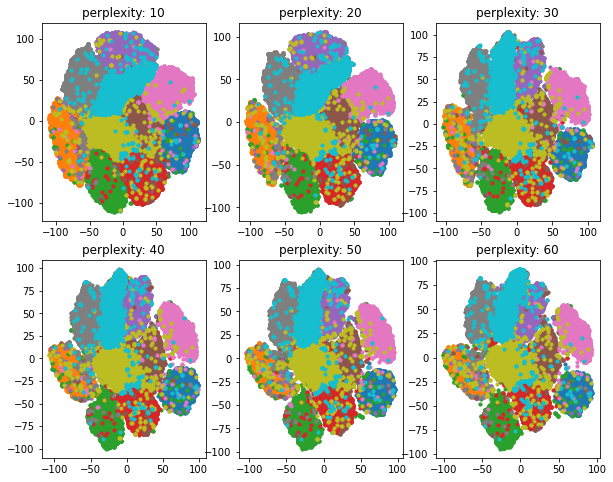
\includegraphics[width=0.6\linewidth]{mnist/tsne_all.png}
    \caption{Αποτελέσματα του t-SNE για διάφορες τιμές του perplexity για τη
    βάση MNIST.}
    \label{fig:mnist_tsne_all}
\end{figure}

\end{frame}

\begin{frame}
\frametitle{Χρόνος εκτέλεσης t-SNE για την MNIST}

\begin{table}[H]
\centering
\begin{tabular}{|c|c|c|c|c|c|c|}
\hline
\textbf{perplexity} & \textbf{10} & \textbf{20} & \textbf{30} & \textbf{40} & \textbf{50} & \textbf{60} \\ \hline
\textbf{seconds}    & 807,75      & 962,41      & 978,5       & 910,81      & 957,05      & 1058,15     \\ \hline
\end{tabular}
\caption{Χρόνος εκτέλεσης του αλγορίθμου t-SNE για διάφορες τιμές του perplexity
    για τη βάση MNIST.}
\label{tab:mnist_tsne_times}
\end{table}

\end{frame}

\begin{frame}
\frametitle{Τελικό αποτέλεσμα t-SNE για την MNIST}

\begin{figure}[H]
    \centering
    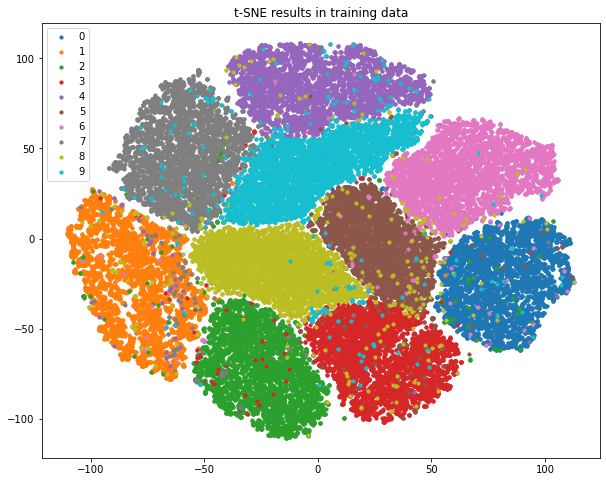
\includegraphics[width=0.6\linewidth]{mnist/tsne_training.png}
    \caption{Αποτελέσμα του t-SNE για την τιμή 10 του perplexity για τη βάση
    MNIST.}
    \label{fig:mnist_tsne}
\end{figure}

\end{frame}

\begin{frame}
\frametitle{Επιλογή παραμέτρων t-SNE για την Cifar-10}

\begin{figure}[H]
    \centering
    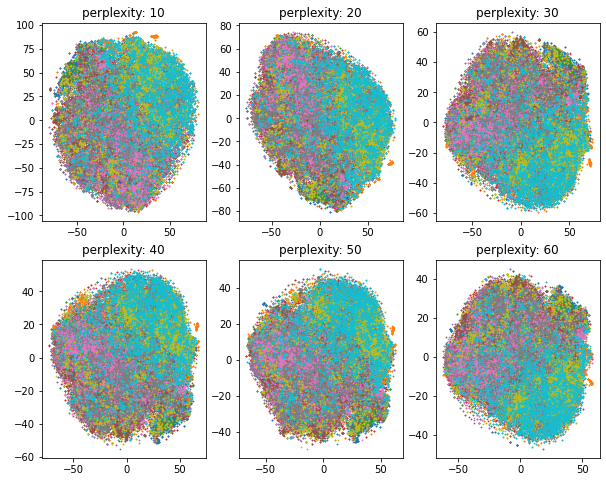
\includegraphics[width=0.6\linewidth]{cifar/tsne_all.png}
    \caption{Αποτελέσματα του t-SNE για διάφορες τιμές του perplexity για τη
    βάση Cifar-10.}
    \label{fig:cifar_tsne_all}
\end{figure}

\end{frame}

\begin{frame}
\frametitle{Χρόνος εκτέλεσης t-SNE για την Cifar-10}

\small
\begin{table}[H]
\centering
\begin{tabular}{|c|c|c|c|c|c|c|}
\hline
\textbf{perplexity} & \textbf{10} & \textbf{20} & \textbf{30} & \textbf{40} & \textbf{50} & \textbf{60} \\ \hline
\textbf{seconds}    & 1024,3      & 1059,65     & 1240,23     & 1337,87     & 1399,87     & 1418,55     \\ \hline
\end{tabular}
\caption{Χρόνος εκτέλεσης του αλγορίθμου t-SNE για διάφορες τιμές του perplexity
    για τη βάση Cifar-10.}
\label{tab:cifar_tsne_times}
\end{table}

\end{frame}

\begin{frame}
\frametitle{Τελικό αποτέλεσμα t-SNE για την Cifar-10}

\begin{figure}[H]
    \centering
    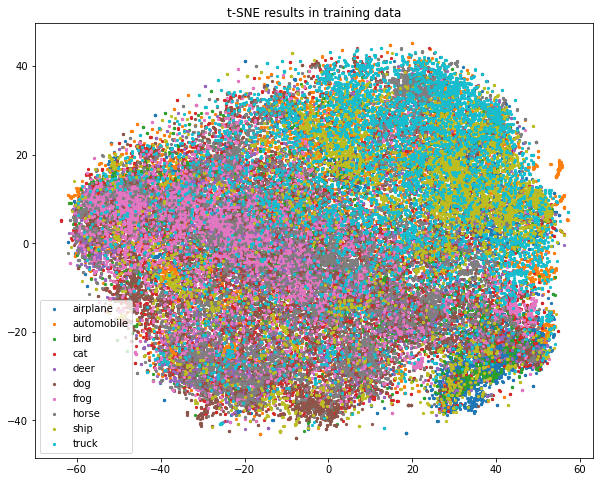
\includegraphics[width=0.6\linewidth]{cifar/tsne_training.png}
    \caption{Αποτελέσμα του t-SNE για την τιμή 60 του perplexity για τη βάση
    Cifar-10.}
    \label{fig:cifar_tsne}
\end{figure}

\end{frame}

\begin{frame}
\frametitle{Επιλογή παραμέτρων spectral clustering για\\την MNIST}

\tiny
\begin{table}[H]
\centering
\begin{tabular}{|c|c|c|c|c|c|c|c|c|}
\hline
\diagbox[innerwidth=2cm]{\textbf{neightbors}}{\textbf{embeddings}} & \textbf{3}      & \textbf{5} & \textbf{8} & \textbf{10} & \textbf{15} & \textbf{20} & \textbf{30} & \textbf{40} \\ \hline
\textbf{15}                                                        & 0,4422          & 0,4995     & 0,6873     & 0,48        & 0,5264      & 0,5454      & 0,3636      & 0,2594      \\ \hline
\textbf{20}                                                        & 0,7461          & 0,6794     & 0,6415     & 0,5709      & 0,6111      & 0,445       & 0,4842      & 0,3278      \\ \hline
\textbf{25}                                                        & 0,7483          & 0,6521     & 0,6004     & 0,5625      & 0,4925      & 0,551       & 0,301       & 0,2694      \\ \hline
\textbf{30}                                                        & 0,7074          & 0,7641     & 0,5954     & 0,5723      & 0,574       & 0,575       & 0,3413      & 0,3748      \\ \hline
\textbf{35}                                                        & 0,7118          & 0,6824     & 0,5969     & 0,621       & 0,5512      & 0,4322      & 0,3866      & 0,3417      \\ \hline
\textbf{40}                                                        & 0,6518          & 0,7695     & 0,6758     & 0,5682      & 0,4976      & 0,5028      & 0,3827      & 0,2743      \\ \hline
\textbf{50}                                                        & \textbf{0,8213} & 0,7845     & 0,674      & 0,6495      & 0,4559      & 0,5478      & 0,3847      & 0,4644      \\ \hline
\end{tabular}
\caption{Αποτελέσματα αναζήτησης πλέγματος της μετρικής ARI για διάφορες τιμές
    των γειτόνων και του αριθμού των embeddings για τη βάση MNIST.}
\label{tab:mnist_grid}
\end{table}

\end{frame}

\begin{frame}
\frametitle{Επιλογή παραμέτρων spectral clustering για\\την Cifar-10}

\tiny
\begin{table}[H]
\centering
\begin{tabular}{|c|c|c|c|c|c|c|c|c|}
\hline
\diagbox[innerwidth=2cm]{\textbf{neightbors}}{\textbf{embeddings}} & \textbf{3} & \textbf{5} & \textbf{8} & \textbf{10} & \textbf{15} & \textbf{20} & \textbf{30} & \textbf{40} \\ \hline
\textbf{10}                                                        & 0,0303     & 0,0475     & 0,0461     & 0,0414      & 0,0379      & 0,0392          & 0,0378      & 0,0311      \\ \hline
\textbf{15}                                                        & 0,0486     & 0,0457     & 0,0476     & 0,0417      & 0,04        & \textbf{0,0488} & 0,0303      & 0,0281      \\ \hline
\textbf{20}                                                        & 0,0464     & 0,0456     & 0,0483     & 0,0413      & 0,0374      & 0,0449          & 0,0356      & 0,0272      \\ \hline
\textbf{25}                                                        & 0,0473     & 0,0456     & 0,0472     & 0,0413      & 0,0367      & 0,0351          & 0,0367      & 0,0124      \\ \hline
\textbf{30}                                                        & 0,0468     & 0,046      & 0,0416     & 0,0413      & 0,0364      & 0,0362          & 0,035       & 0,0275      \\ \hline
\textbf{40}                                                        & 0,0485     & 0,0447     & 0,0474     & 0,0481      & 0,0427      & 0,0482          & 0,0351      & 0,0253      \\ \hline
\textbf{50}                                                        & 0,0449     & 0,0459     & 0,0402     & 0,0403      & 0,0362      & 0,0354          & 0,029       & 0,023       \\ \hline
\end{tabular}
\caption{Αποτελέσματα αναζήτησης πλέγματος της μετρικής ARI για διάφορες τιμές
    των γειτόνων και του αριθμού των embeddings για τη βάση Cifar-10.}
\label{tab:cifar_grid}
\end{table}

\end{frame}

\begin{frame}
\frametitle{Αποτέλεσμα καλύτερου μοντέλου στην MNIST}

\begin{figure}[H]
    \centering
    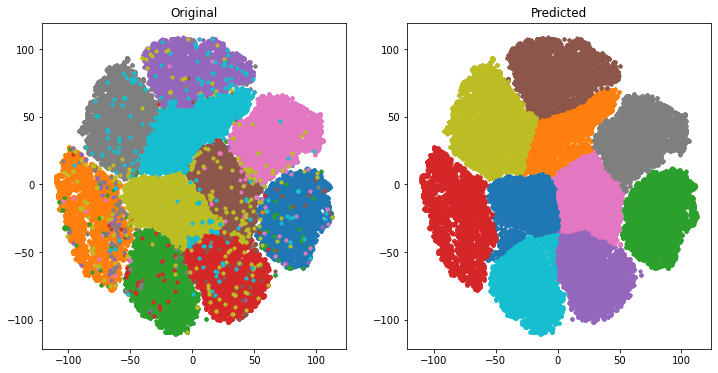
\includegraphics[width=0.8\linewidth]{mnist/best_model_results.png}
    \caption{Αποτέλεσμα ομαδοποίησης του καλύτερου μοντέλου σε σχέση με τις
    πραγματικές κλάσεις για τη βάση MNIST.}
    \label{fig:mnist_best_model_results}
\end{figure}

\end{frame}

\begin{frame}
\frametitle{Ιδιοτιμές καλύτερου μοντέλου στην MNIST}

\begin{figure}[H]
    \centering
    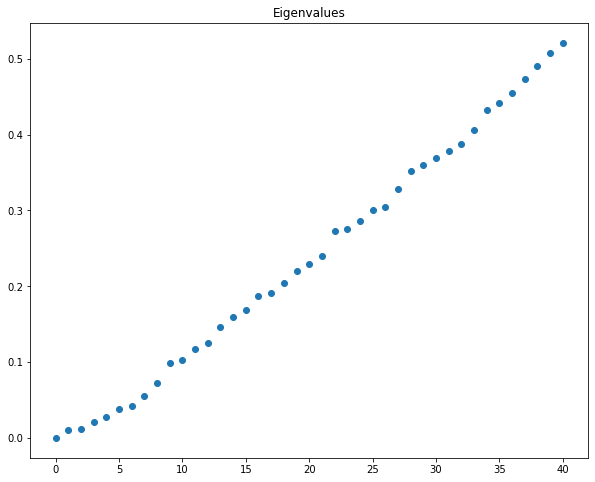
\includegraphics[width=0.6\linewidth]{mnist/eigenvalues.png}
    \caption{Ιδιοτιμές του καλύτερου μοντέλου για τη βάση MNIST.}
    \label{fig:mnist_eigenvalues}
\end{figure}

\end{frame}

\begin{frame}
\frametitle{Αποτελέσματα καλύτερου μοντέλου στην MNIST\\για διάφορες τιμές
    γειτόνων}

\begin{figure}[H]
    \centering
    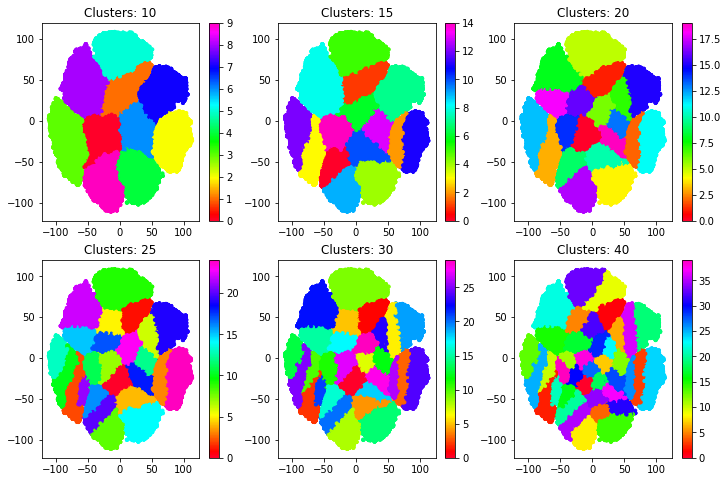
\includegraphics[width=0.8\linewidth]{mnist/dif_clusters.png}
    \caption{Αποτελέσματα για διάφορες τιμές του αριθμού των ομάδων για τη βάση
    MNIST.}
    \label{fig:mnist_dif_clusters}
\end{figure}

\end{frame}

\begin{frame}
\frametitle{Αποτελέσματα καλύτερου μοντέλου στην MNIST\\για διάφορες τιμές
    γειτόνων}

\small
\begin{table}[H]
\centering
\begin{tabular}{|c|c|c|c|c|c|c|}
\hline
\diagbox[innerwidth=2cm]{\textbf{Data}}{\textbf{Clusters}} & \textbf{10} & \textbf{15} & \textbf{20} & \textbf{25} & \textbf{30} & \textbf{40} \\ \hline
\textbf{Embeddings}                                        & 0,5244      & 0,5023      & 0,4926      & 0,4699      & 0,4492      & 0,4159      \\ \hline
\textbf{TSNE 2D space}                                     & 0,3632      & 0,3067      & 0,2639      & 0,258       & 0,257       & 0,2564      \\ \hline
\end{tabular}
\caption{Αποτελέσματα μετρικής silhouette με βάση τις αποστάσεις των embeddings
    και τις αποστάσεις στις δύο διαστάσεις για τη βάση MNIST.}
\label{tab:mnist_sil}
\end{table}

\end{frame}








\begin{frame}
\frametitle{Αποτέλεσμα καλύτερου μοντέλου στην Cifar-10}

\begin{figure}[H]
    \centering
    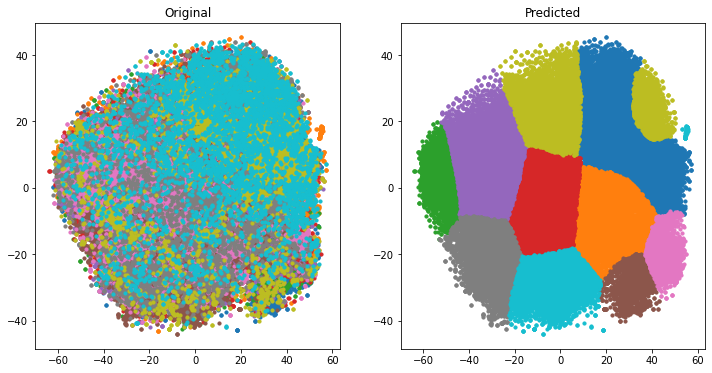
\includegraphics[width=0.8\linewidth]{cifar/best_model_results.png}
    \caption{Αποτέλεσμα ομαδοποίησης του καλύτερου μοντέλου σε σχέση με τις
    πραγματικές κλάσεις για τη βάση Cifar-10.}
    \label{fig:cifar_best_model_results}
\end{figure}

\end{frame}

\begin{frame}
\frametitle{Ιδιοτιμές καλύτερου μοντέλου στην Cifar-10}

\begin{figure}[H]
    \centering
    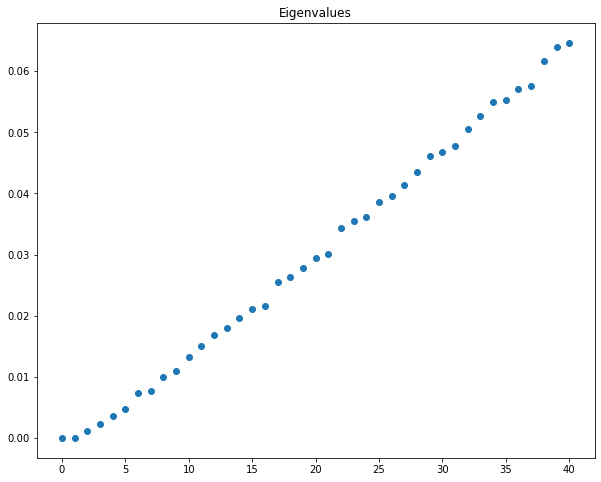
\includegraphics[width=0.6\linewidth]{cifar/eigenvalues.png}
    \caption{Ιδιοτιμές του καλύτερου μοντέλου για τη βάση Cifar-10.}
    \label{fig:cifar_eigenvalues}
\end{figure}

\end{frame}

\begin{frame}
\frametitle{Αποτελέσματα καλύτερου μοντέλου στην Cifar-10\\για διάφορες τιμές
    γειτόνων}

\begin{figure}[H]
    \centering
    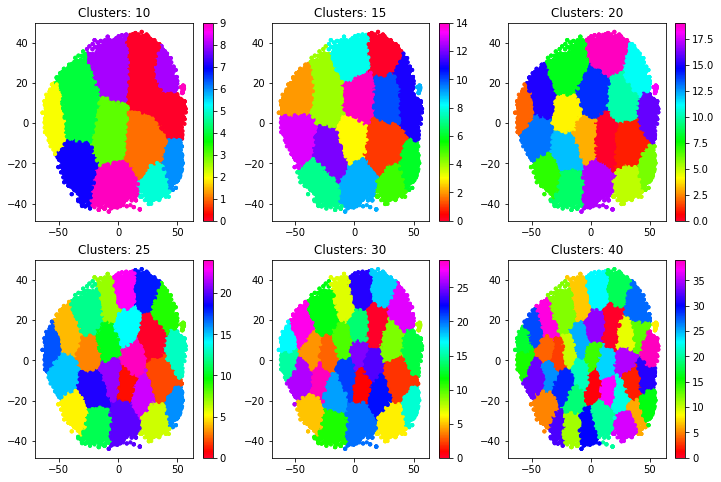
\includegraphics[width=0.8\linewidth]{cifar/dif_clusters.png}
    \caption{Αποτελέσματα για διάφορες τιμές του αριθμού των ομάδων για τη βάση
    Cifar-10.}
    \label{fig:cifar_dif_clusters}
\end{figure}

\end{frame}

\begin{frame}
\frametitle{Αποτελέσματα καλύτερου μοντέλου στην Cifar-10\\για διάφορες τιμές
    γειτόνων}

\small
\begin{table}[H]
\centering
\begin{tabular}{|c|c|c|c|c|c|c|}
\hline
\diagbox[innerwidth=2cm]{\textbf{Data}}{\textbf{Clusters}} & \textbf{10} & \textbf{15} & \textbf{20} & \textbf{25} & \textbf{30} & \textbf{40} \\ \hline
\textbf{Embeddings}                                        & 0,5244      & 0,5023      & 0,4926      & 0,4699      & 0,4492      & 0,4159      \\ \hline
\textbf{TSNE 2D space}                                     & 0,3632      & 0,3067      & 0,2639      & 0,258       & 0,257       & 0,2564      \\ \hline
\end{tabular}
\caption{Αποτελέσματα μετρικής silhouette με βάση τις αποστάσεις των embeddings
    και τις αποστάσεις στις δύο διαστάσεις για τη βάση Cifar-10.}
\label{tab:cifar_sil}
\end{table}

\end{frame}


\begin{frame}[allowframebreaks]
\frametitle{Βιβλιογραφία}

\begin{english}
\printbibliography[title=Βιβλιογραφία]
\end{english}

\end{frame}


\begin{frame}
\frametitle{Ερωτήσεις}

\begin{figure}[H]
    \centering
    \includegraphics[height=0.8\textheight]{question_mark}
\end{figure}

\end{frame}


\end{document}
